\documentclass[Afour,sagev,times]{sagej}

\usepackage{moreverb,url}
\usepackage{graphicx}
\usepackage{amsmath}
\usepackage{amssymb}
\usepackage{array}
\usepackage{booktabs}
\usepackage{placeins}
\usepackage[colorlinks,bookmarksopen,bookmarksnumbered,citecolor=red,urlcolor=red]{hyperref}

% Chinese translation support for Overleaf.
% Please compile this bilingual version with XeLaTeX.
\usepackage{fontspec}
\usepackage{xeCJK}
\setmainfont{TeX Gyre Termes}
\setsansfont{TeX Gyre Heros}
\setmonofont{TeX Gyre Cursor}
\xeCJKsetup{AutoFakeBold=true,AutoFakeSlant=true}
\setCJKmainfont[
  BoldFont=FandolHei-Regular,
  ItalicFont=FandolKai-Regular,
  BoldItalicFont=FandolHei-Regular
]{FandolSong-Regular}
\setCJKsansfont{FandolHei-Regular}
\setCJKmonofont{FandolFang-Regular}

\newcommand\BibTeX{{\rmfamily B\kern-.05em \textsc{i\kern-.025em b}\kern-.08em
T\kern-.1667em\lower.7ex\hbox{E}\kern-.125emX}}

\def\volumeyear{2026}

\begin{document}

\runninghead{Lin et al.}

\title{Multimodal endoscopic finding-guided cross-attentive hypergraph multiple instance learning for examination-level multi-label classification of gastroscopy examinations: a retrospective single-center study}

\author{Zijian Lin\affilnum{1,2}, Chengze Cai\affilnum{3}, Chenxi Huang\affilnum{2}, Hua Gao\affilnum{1} and Jie He\affilnum{1,4}}

\affiliation{\affilnum{1}Department of Endoscopy Center, Zhongshan Hospital (Xiamen), Fudan University, Xiamen 361015, China\\
\affilnum{2}School of Informatics, Xiamen University, Xiamen, Fujian 361102, China\\
\affilnum{3}College of Computer and Information Sciences, Fujian Agriculture and Forestry University, Fuzhou, Fujian 350002, China\\
\affilnum{4}Xiamen Clinical Research Center for Cancer Therapy, Xiamen 361015, China}

\corrauth{Hua Gao and Jie He, Department of Endoscopy Center, Zhongshan Hospital (Xiamen), Fudan University, 668 Jinhu Road, Huli District, Xiamen, Fujian 361015, China.}

\email{208908636@qq.com; gao.hua@zsxmhospital.com; he.jie@zsxmhospital.com}

\begin{abstract}
\textbf{OBJECTIVE:} To develop and internally validate a report-assisted multimodal weakly supervised framework for examination-level multi-label classification of routine gastroscopy examinations, focusing on esophageal submucosal tumor, esophageal mucosal lesion, and gastritis. \textbf{METHODS:} This retrospective single-center study included 2872 eligible gastroscopy examinations from 2272 patients, comprising 171991 endoscopic images. Examination-level labels were derived from the diagnostic conclusion field, whereas this label-derivation field was not used as model input. We proposed \textit{MEF-CAH-MIL} (Multimodal Endoscopic Finding-Guided Cross-Attentive Hypergraph Multiple Instance Learning), a multimodal MIL framework that represents each examination as a long-context image bag and integrates the routine endoscopic finding text field (\textit{watch}) through label-query cross-attention. The framework combines a ConvNeXt-Tiny image encoder, 64-instance MIL aggregation, a lightweight hashed-token text encoder, gated multimodal residual fusion, and label hypergraph reasoning for coexisting findings. The cohort was split with patient grouping into training, validation, and test sets; minority-label oversampling was applied only to the training set. The model was evaluated on a fixed internal test set of 567 examinations. \textbf{RESULTS:} The best macro-F1 checkpoint achieved a macro F1 of 0.8979, micro F1 of 0.8949, macro ROC-AUC of 0.9532, macro PR-AUC of 0.9362, subset accuracy of 0.7813, hamming loss of 0.1029, and Cohen's kappa of 0.7945. Label-wise F1 scores were 0.8766 for esophageal submucosal tumor, 0.8787 for esophageal mucosal lesion, and 0.9384 for gastritis. \textbf{CONCLUSIONS:} \textit{MEF-CAH-MIL} offers a practical route for integrating multi-image gastroscopy evidence with routine endoscopic finding text at the examination level. The results support the feasibility of multimodal examination-level decision support, but they should not be interpreted as pure image-only diagnostic performance because the \textit{watch} field is available during inference. External validation, prospective workflow evaluation, and careful leakage auditing remain necessary before clinical deployment.

\textbf{中文翻译：} 目的：开发并内部验证一种报告辅助的多模态弱监督框架，用于常规胃镜检查级多标签分类，重点识别食管黏膜下肿瘤、食管粘膜病变以及胃炎。方法：本回顾性单中心研究纳入来自2272名患者的2872次符合条件胃镜检查，共包含171991张内镜图像。检查级标签由诊断结论字段生成，而该标签派生字段不作为模型输入。本文提出\textit{MEF-CAH-MIL}（Multimodal Endoscopic Finding-Guided Cross-Attentive Hypergraph Multiple Instance Learning）多模态多实例学习框架，将每次检查表示为长上下文图像bag，并通过标签查询cross-attention融合常规内镜所见文本字段（\textit{watch}）。该框架结合ConvNeXt-Tiny图像编码器、64实例MIL聚合、轻量级哈希token文本编码器、门控多模态残差融合以及用于共存发现建模的标签超图推理模块。队列按患者分组划分为训练集、验证集和测试集；少数标签过采样仅用于训练集。模型在固定内部测试集567次检查上进行评估。结果：最佳宏平均F1 checkpoint取得0.8979的宏平均F1、0.8949的微平均F1、0.9532的宏平均ROC-AUC、0.9362的宏平均PR-AUC、0.7813的子集准确率、0.1029的汉明损失和0.7945的Cohen's kappa。三个标签的F1分别为：食管黏膜下肿瘤0.8766、食管粘膜病变0.8787、胃炎0.9384。结论：\textit{MEF-CAH-MIL}为在检查级别融合多图像胃镜证据和常规内镜所见文本提供了一条实用路径。结果支持多模态检查级决策支持的可行性，但由于推理阶段使用\textit{watch}字段，不能将其解释为纯图像诊断性能。临床部署前仍需外部验证、前瞻性工作流评估和严格的数据泄漏审计。
\end{abstract}

\keywords{gastroscopy, examination-level classification, multimodal learning, endoscopic finding-guided learning, cross-attentive hypergraph multiple instance learning, report-assisted decision support}

\maketitle

\noindent\textbf{中文翻译：} 关键词：胃镜检查，检查级分类，多模态学习，内镜所见引导学习，交叉注意力超图多实例学习，报告辅助决策支持

\medskip

\section{Introduction}

Upper gastrointestinal endoscopy is widely used to examine abnormalities of the esophagus and stomach. A gastroscopy examination contains a sequence of images acquired from different anatomical sites and viewing angles. A focal lesion may appear in only a few images, whereas diffuse inflammation may be visible across multiple images. In this study, we focus on three diseases that can be identified during upper gastrointestinal endoscopy: esophageal submucosal tumor, esophageal mucosal lesion, and gastritis. Esophageal submucosal tumors arise beneath the mucosal surface and often appear as smooth, localized elevations with relatively intact overlying mucosa. Esophageal mucosal lesions involve visible abnormalities of the mucosal surface, such as changes in color, erosion, or irregular morphology. Gastritis refers to inflammation of the gastric mucosa and may appear as erythema, edema, erosion, or other diffuse mucosal changes.

\noindent\textbf{中文翻译：}
上消化道内镜被广泛用于检查食管和胃部异常。一次胃镜检查包含从不同解剖部位和观察角度采集的一系列图像。局灶性病变可能只出现在少数图像中，而弥漫性炎症可能出现在多张图像中。本文关注三个在上消化道内镜检查中可以发现的疾病：食管黏膜下肿瘤、食管粘膜病变和胃炎。食管黏膜下肿瘤起源于黏膜表面下方，在内镜下通常表现为表面黏膜相对完整的光滑局灶性隆起。食管粘膜病变是食管粘膜表面的可见异常，可表现为色泽改变、糜烂或形态不规则。胃炎是胃黏膜的炎症改变，可表现为充血、红斑、水肿、糜烂或其他弥漫性黏膜异常。

Most publicly available gastroscopy datasets are constructed at the image level and contain selected lesion images paired with category labels.\cite{R4,R5,R21} Creating these datasets requires clinicians to inspect and annotate individual images, which is time-consuming and limits the scale of the data. Manual selection also favors clear and typical lesions, while a single image-level category may not accurately describe the transition or boundary between a lesion and normal tissue, leading to selection bias and label noise. Treating each image independently further ignores the acquisition order and contextual relationships among images from the same examination. Public datasets that retain complete examination sequences remain limited, and relatively few studies have investigated which diseases are present across a complete gastroscopy examination. Examination-level learning uses labels assigned to the complete examination, reducing image-by-image annotation while preserving the examination context.

\noindent\textbf{中文翻译：}
现有公开胃镜数据集大多以图像级形式构建，包含经过筛选的病灶图像及其类别标签。\cite{R4,R5,R21} 构建这类数据集需要医生逐张查看并标注图像，不仅耗时，也限制了数据集规模。人工筛选还容易偏向清晰、典型的病灶，而单一的图像级类别难以准确描述病灶与正常组织之间的过渡或边界区域，从而带来选择偏差和标签噪声。将每张图像独立处理还会忽略同一次检查中图像的采集顺序和上下文关系。目前，保留完整检查序列的公开数据集仍然较少，研究一次完整胃镜检查中存在哪些疾病的工作也相对有限。检查级学习使用完整检查对应的标签，可以减少逐图标注，同时保留检查上下文。

Multiple instance learning (MIL) is suitable for examination-level learning because it treats each examination as an image bag and learns from bag-level labels.\cite{R6,R7,R8,R9,R10,R22} However, conventional MIL usually treats images as unordered instances and compresses them into a single bag representation. It therefore does not explicitly model image order or inter-image dependencies within an examination. A shared bag representation is also limited for multi-label prediction because different diseases may be supported by different images. In addition, many multi-label methods predict each label independently or model only pairwise label relationships, which may not fully capture the higher-order relationships among several coexisting diseases.\cite{R14,R18} Moreover, existing examination-level MIL methods generally learn only from visual instances and do not fully exploit the semantic descriptions of lesion appearance and location in physician-written clinical diagnostic reports, limiting the use of complementary image-text information for examination-level disease representation.

\noindent\textbf{中文翻译：}
多实例学习（MIL）适合检查级学习，因为它将每次检查视为一个图像 bag，并利用 bag 级标签进行学习。\cite{R6,R7,R8,R9,R10,R22} 然而，传统 MIL 通常将图像视为无序实例，并将其压缩为一个整体 bag 表征，因此没有显式建模检查内图像的顺序和图像间依赖关系。共享的 bag 表征也不利于多标签预测，因为不同疾病可能由不同图像提供证据。此外，许多多标签方法独立预测各个标签，或只建模标签之间的两两关系，难以充分捕获多个共存疾病之间的高阶关系。\cite{R14,R18} 此外，现有检查级 MIL 方法通常只从视觉实例中学习，没有充分利用医生临床诊断报告中关于病灶形态和位置的语义描述，因而难以利用图像与文本的互补信息形成更完整的检查级疾病表征。

To address these limitations, we construct an examination-level multimodal gastroscopy dataset. Each examination contains a complete image sequence, examination-level labels for the three diseases, and a clinical diagnostic report written by a physician to describe lesion appearance and location. This structure avoids image-by-image annotation while preserving both examination context and report semantics. To reduce direct label leakage, target category names in the reports are masked before text encoding. Based on this dataset, we propose \textit{MEF-CAH-MIL} (\textbf{M}ultimodal \textbf{E}ndoscopic \textbf{F}inding-Guided \textbf{C}ross-\textbf{A}ttentive \textbf{H}ypergraph \textbf{M}ultiple \textbf{I}nstance \textbf{L}earning). The model uses a position-aware Transformer to capture image order and inter-image relationships, multi-label attention MIL to aggregate disease-specific visual evidence, and a label hypergraph reasoner to model higher-order relationships among coexisting diseases. Label-query cross-attention and gated fusion connect each disease with relevant content in the masked report. The full multimodal pathway serves as the main classification branch, while an image-only branch is retained to produce predictions based solely on visual evidence.

\noindent\textbf{中文翻译：}
为解决上述问题，本文构建了一套检查级多模态胃镜数据集。每次检查包含完整图像序列、三个疾病的检查级标签，以及由医生书写并描述病灶表现和病灶区域的临床诊断报告。该数据结构无需逐图标注，同时保留了检查上下文和报告语义。为减少直接的标签信息泄露，报告中的目标类别名称会在文本编码前被掩码。基于该数据集，本文提出 \textit{MEF-CAH-MIL}（\textbf{M}ultimodal \textbf{E}ndoscopic \textbf{F}inding-Guided \textbf{C}ross-\textbf{A}ttentive \textbf{H}ypergraph \textbf{M}ultiple \textbf{I}nstance \textbf{L}earning）。该模型使用位置感知 Transformer 捕获图像顺序和图像间关系，使用多标签注意力 MIL 聚合疾病特异性视觉证据，并通过标签超图推理器建模多个共存疾病之间的高阶关系。标签查询 cross-attention 和门控融合机制将每种疾病与掩码报告中的相关内容联系起来。模型以包含全部模块的多模态路径作为主分类分支，同时保留纯图像分支，用于生成仅基于视觉证据的预测结果。

The main contributions of this study are summarized as follows:
\begin{itemize}
    \item We construct an examination-level multimodal gastroscopy dataset that contains complete image sequences, examination-level multi-label annotations, and physician-written clinical diagnostic reports. This dataset supports weakly supervised examination-level learning without requiring image-by-image annotation.
    \item We propose a position-aware Transformer to model image order and inter-image dependencies within a complete examination, enabling the model to integrate visual evidence distributed across the examination sequence.
    \item We develop multi-label attention MIL to aggregate different image evidence for each disease and a label hypergraph reasoner to capture higher-order relationships among coexisting diseases.
    \item We introduce label-query cross-attention and gated fusion to connect label-specific visual evidence with category-masked report content. The full multimodal pathway serves as the main branch, while the retained image-only branch enables separate evaluation of predictions based solely on visual evidence.
\end{itemize}

\noindent\textbf{中文翻译：}
本文的主要贡献总结如下：
\begin{itemize}
    \item 本文构建了一套检查级多模态胃镜数据集，其中包含完整检查图像序列、检查级多标签标注以及医生书写的临床诊断报告。该数据集支持无需逐图标注的检查级弱监督学习。
    \item 本文提出位置感知 Transformer，用于建模完整检查中的图像顺序和图像间依赖关系，使模型能够整合分布在检查序列中的视觉证据。
    \item 本文设计多标签注意力 MIL，为每种疾病聚合不同的图像证据，并通过标签超图推理器捕获多个共存疾病之间的高阶关系。
    \item 本文引入标签查询 cross-attention 和门控融合机制，将标签特异性视觉证据与经过类别名称掩码的报告内容联系起来。包含全部模块的多模态路径作为主分支，同时保留纯图像分支，以单独评估仅基于视觉证据的预测结果。
\end{itemize}

\section{Related Work}

\subsection{Endoscopic Datasets and Examination-Level Multi-Image Learning}

Public gastrointestinal endoscopy datasets have mainly supported image-level recognition. Kvasir provides labeled images from predefined anatomical and pathological categories, while HyperKvasir expands the scale to labeled images, unlabeled images, and videos.\cite{R4,R5} These datasets enabled reproducible comparisons of image classification methods, but their commonly used labeled subsets are still organized mainly by image or video category.\cite{R21} Based on such data, Takiyama et al. classified anatomical sites from individual upper gastrointestinal endoscopy images, whereas Hirasawa et al. and Luo et al. detected upper gastrointestinal cancer from selected images or video frames.\cite{R2,R3,R19} Wu et al. developed WISENSE to monitor blind spots during upper gastrointestinal endoscopy, showing the value of procedural information for quality control rather than examination-level multi-label disease classification.\cite{R20} To reduce the need for manual image annotation, Buendgens et al. linked routine gastroscopy and colonoscopy images to examination-level diagnoses and aggregated image predictions at the examination level, showing the feasibility of weakly supervised learning from routine archives.\cite{R25} More recently, GastroHUN provided patient-linked images and short sequences collected under a systematic stomach screening protocol, offering an important benchmark for anatomical image and sequence classification.\cite{R26} Nevertheless, public datasets and studies for multi-label disease classification from complete gastroscopy examinations remain limited. Existing examination-level methods also rarely model the acquisition order, relative positions, and dependencies among all images in an examination. Our work addresses these gaps by constructing an examination-level multimodal dataset and explicitly modeling position-aware relationships within each image bag.

\noindent\textbf{中文翻译：}
现有胃肠内镜公开数据集主要支持图像级识别。Kvasir 提供预定义解剖部位和病理类别的标注图像，HyperKvasir 则进一步扩展到标注图像、未标注图像和视频。\cite{R4,R5} 这些数据集推动了图像分类方法的可重复比较，但其常用标注子集仍主要按照图像或视频类别组织。\cite{R21} 基于这类数据，Takiyama 等人对单张上消化道内镜图像进行解剖部位分类，Hirasawa 等人和 Luo 等人则从筛选图像或视频帧中检测上消化道癌。\cite{R2,R3,R19} Wu 等人开发 WISENSE 监测上消化道内镜检查中的盲区，说明检查流程信息可以用于质量控制，但该任务并非检查级多标签疾病分类。\cite{R20} 为减少人工图像标注，Buendgens 等人将常规胃镜和结肠镜图像与检查级诊断相匹配，并在检查级聚合图像预测，证明了从常规归档数据进行弱监督学习的可行性。\cite{R25} 最近，GastroHUN 提供了按照系统性胃部筛查流程采集的患者关联图像和短序列，为解剖部位的图像和序列分类提供了重要基准。\cite{R26} 尽管取得了这些进展，面向完整胃镜检查的多标签疾病分类公开数据和相关研究仍然有限。现有检查级方法也很少同时建模一次检查中全部图像的采集顺序、相对位置和图像间依赖关系。针对这些不足，本文构建检查级多模态数据集，并显式建模图像 bag 内的位置感知关系。

\subsection{Multi-Label MIL and Higher-Order Label Reasoning}

MIL provides a practical solution when a case has a bag-level label but its individual instances are not annotated. Ilse et al. proposed attention-based MIL to learn a weighted bag representation, providing a trainable way to identify informative instances.\cite{R6} CLAM introduced clustering constraints to separate instance-level evidence, DSMIL combined instance and bag classifiers, TransMIL used Transformer attention to model instance correlations, and DTFD-MIL improved learning from large bags through feature distillation.\cite{R7,R8,R9,R10} These methods have advanced weakly supervised medical image analysis, especially for pathology slides, but they generally produce one overall bag representation for prediction. In an examination-level multi-label task, this shared representation may mix evidence because different diseases can appear in different images. Multi-label classification further requires modeling dependencies among labels. Asymmetric loss improves learning under class imbalance, but it does not explicitly connect each label to its supporting instances or model label relations.\cite{R12} Chen et al. used a graph convolutional network to build interdependent label classifiers from pairwise co-occurrence, while Feng et al. showed that hypergraphs can represent higher-order relationships through hyperedges connecting multiple nodes.\cite{R14,R18} However, label-specific image aggregation and higher-order label reasoning have not been jointly studied for multi-label classification of complete gastroscopy examinations. Our method therefore combines multi-label attention MIL with a label hypergraph reasoner so that each disease can collect its own visual evidence and exchange information through higher-order label relations.

\noindent\textbf{中文翻译：}
当一个病例只有 bag 级标签而缺少实例标注时，MIL 提供了一种实用的解决方案。Ilse 等人提出注意力 MIL，通过学习加权的 bag 表征识别重要实例。\cite{R6} CLAM 引入聚类约束以区分实例级证据，DSMIL 结合实例分类器和 bag 分类器，TransMIL 使用 Transformer 注意力建模实例相关性，DTFD-MIL 则通过特征蒸馏改善超大 bag 的学习。\cite{R7,R8,R9,R10} 这些方法推动了弱监督医学图像分析，尤其是病理全切片分析，但通常仍生成一个整体 bag 表征用于预测。在检查级多标签任务中，不同疾病可能出现在不同图像中，共享表征容易混合不同疾病的证据。多标签分类还需要建模标签之间的依赖关系。Asymmetric loss 能够改善类别不平衡条件下的学习，但不能显式建立标签与其支持实例之间的联系，也不负责建模标签关系。\cite{R12} Chen 等人使用图卷积网络，根据标签的两两共现关系构建相互依赖的分类器；Feng 等人则表明，超图可以通过连接多个节点的超边表示高阶关系。\cite{R14,R18} 然而，标签特异性图像聚合与高阶标签推理尚未在完整胃镜检查的多标签分类中得到联合研究。因此，本文将多标签注意力 MIL 与标签超图推理器结合，使每种疾病能够聚合各自的视觉证据，并通过高阶标签关系进行信息交互。

\subsection{Report-Guided Multimodal Medical Image Learning}

Image-text learning provides a way to use semantic information from clinical reports. In general vision-language learning, ALBEF aligns image and text representations before fusion, while BLIP improves multimodal pretraining through caption generation and filtering.\cite{R15,R16} In medical imaging, ConVIRT learns visual representations from paired images and reports through contrastive learning, GLoRIA introduces global and local alignment between radiographs and report text, and REFERS uses cross-supervision between images and free-text reports.\cite{R23,R17,R24} These methods show that report semantics can improve medical visual representation learning. However, most of them align an image or image set with a report at a global or regional level. A clinical report may describe several findings, so global alignment does not directly determine which text content and which images support each disease label. Using diagnostic reports as model inputs also creates a risk of direct label leakage when target category names appear in the text. Existing report-guided methods do not directly address label-specific text retrieval, category-name masking, and examination-level MIL within one framework. Our method uses label-query cross-attention to retrieve relevant content from category-masked reports and gated fusion to control its contribution. The full multimodal pathway is used as the main branch, while a retained image-only branch allows visual predictions to be evaluated separately.

\noindent\textbf{中文翻译：}
图文学习为利用临床报告中的语义信息提供了一种方法。在通用视觉语言学习中，ALBEF 在融合前对齐图像和文本表征，BLIP 则通过图像描述生成与筛选改进多模态预训练。\cite{R15,R16} 在医学影像领域，ConVIRT 通过对比学习从配对图像和报告中学习视觉表征，GLoRIA 建立放射图像与报告文本之间的全局和局部对齐，REFERS 则利用图像和自由文本报告之间的交叉监督。\cite{R23,R17,R24} 这些方法表明，报告语义能够帮助医学视觉表征学习。然而，这些方法大多在全局或局部区域层面对图像与报告进行对齐。一份临床报告可能描述多个发现，因此全局对齐无法直接确定哪些文本内容和哪些图像为每个疾病标签提供证据。当诊断报告中出现目标类别名称时，将报告作为模型输入还可能造成直接的标签信息泄露。现有报告引导方法尚未在一个框架中同时解决标签特异性文本检索、类别名称掩码和检查级 MIL。本文使用标签查询 cross-attention 从经过类别名称掩码的报告中检索相关内容，并通过门控融合控制文本信息的作用。模型以完整多模态路径作为主分支，同时保留纯图像分支，以单独评估视觉预测结果。
\section{Materials and Methods}

\subsection{Dataset construction and preprocessing}

\subsubsection{Study design and source data}

This retrospective observational study used de-identified clinical data from Zhongshan Hospital (Xiamen), Fudan University. The study population consisted of patients who underwent gastroscopy at the hospital and whose examination records passed the data integrity and report-level screening procedures described below. The source data included an institutional endoscopy image archive, structured endoscopy reports, and related fields from the hospital's internal clinical database. The collaborating hospital agreed that the de-identified clinical archive could be used for this research. Because the data may contain sensitive clinical information and are subject to hospital data governance requirements, the raw data are not publicly available; access to de-identified derived data may be considered upon reasonable request to the corresponding author and with permission from the hospital.

\textbf{中文翻译：} 本研究为一项回顾性观察性研究，使用来自复旦大学附属中山医院厦门医院的去标识化临床数据。研究对象为在该院接受胃镜检查，并通过下述数据完整性检查和报告级筛选流程的患者。数据来源包括院内内镜图像归档、结构化内镜报告以及医院内部临床数据库中的相关字段。合作医院同意将该去标识化临床归档数据用于本研究。由于数据可能包含敏感临床信息，并受医院数据管理规定约束，本研究所用原始数据不公开；经合理申请并获得医院许可后，可向通讯作者申请获取去标识化派生数据。

To clarify how routine clinical archive data were transformed into model-ready samples, we organized dataset construction into three stages: raw image-report collection, data cleaning and report-derived multi-label generation, and examination-level multimodal sample construction. The diagnostic conclusion field was used only to derive examination-level labels and was not provided to the model. Each final sample contained a sampled image bag with a valid-image mask and the matched endoscopic finding text. Before entering the text branch, direct target-category expressions in the finding text were masked to reduce label leakage. The complete workflow is summarized in Figure~\ref{fig:dataset_pipeline}.

\textbf{中文翻译：} 为了说明常规临床归档数据如何转化为模型可用样本，本文将数据集构建分为三个阶段：原始图像与报告收集、数据清洗和基于报告的多标签生成，以及检查级多模态样本构建。诊断结论字段仅用于生成检查级标签，不提供给模型。每个最终样本包含带有效图像掩码的采样图像bag和与之匹配的内镜所见文本；文本进入模型前，对其中直接提示目标类别的表述进行掩码，以减少标签信息泄露。完整的数据处理流程见图~\ref{fig:dataset_pipeline}。

\begin{figure*}[t]
\centering
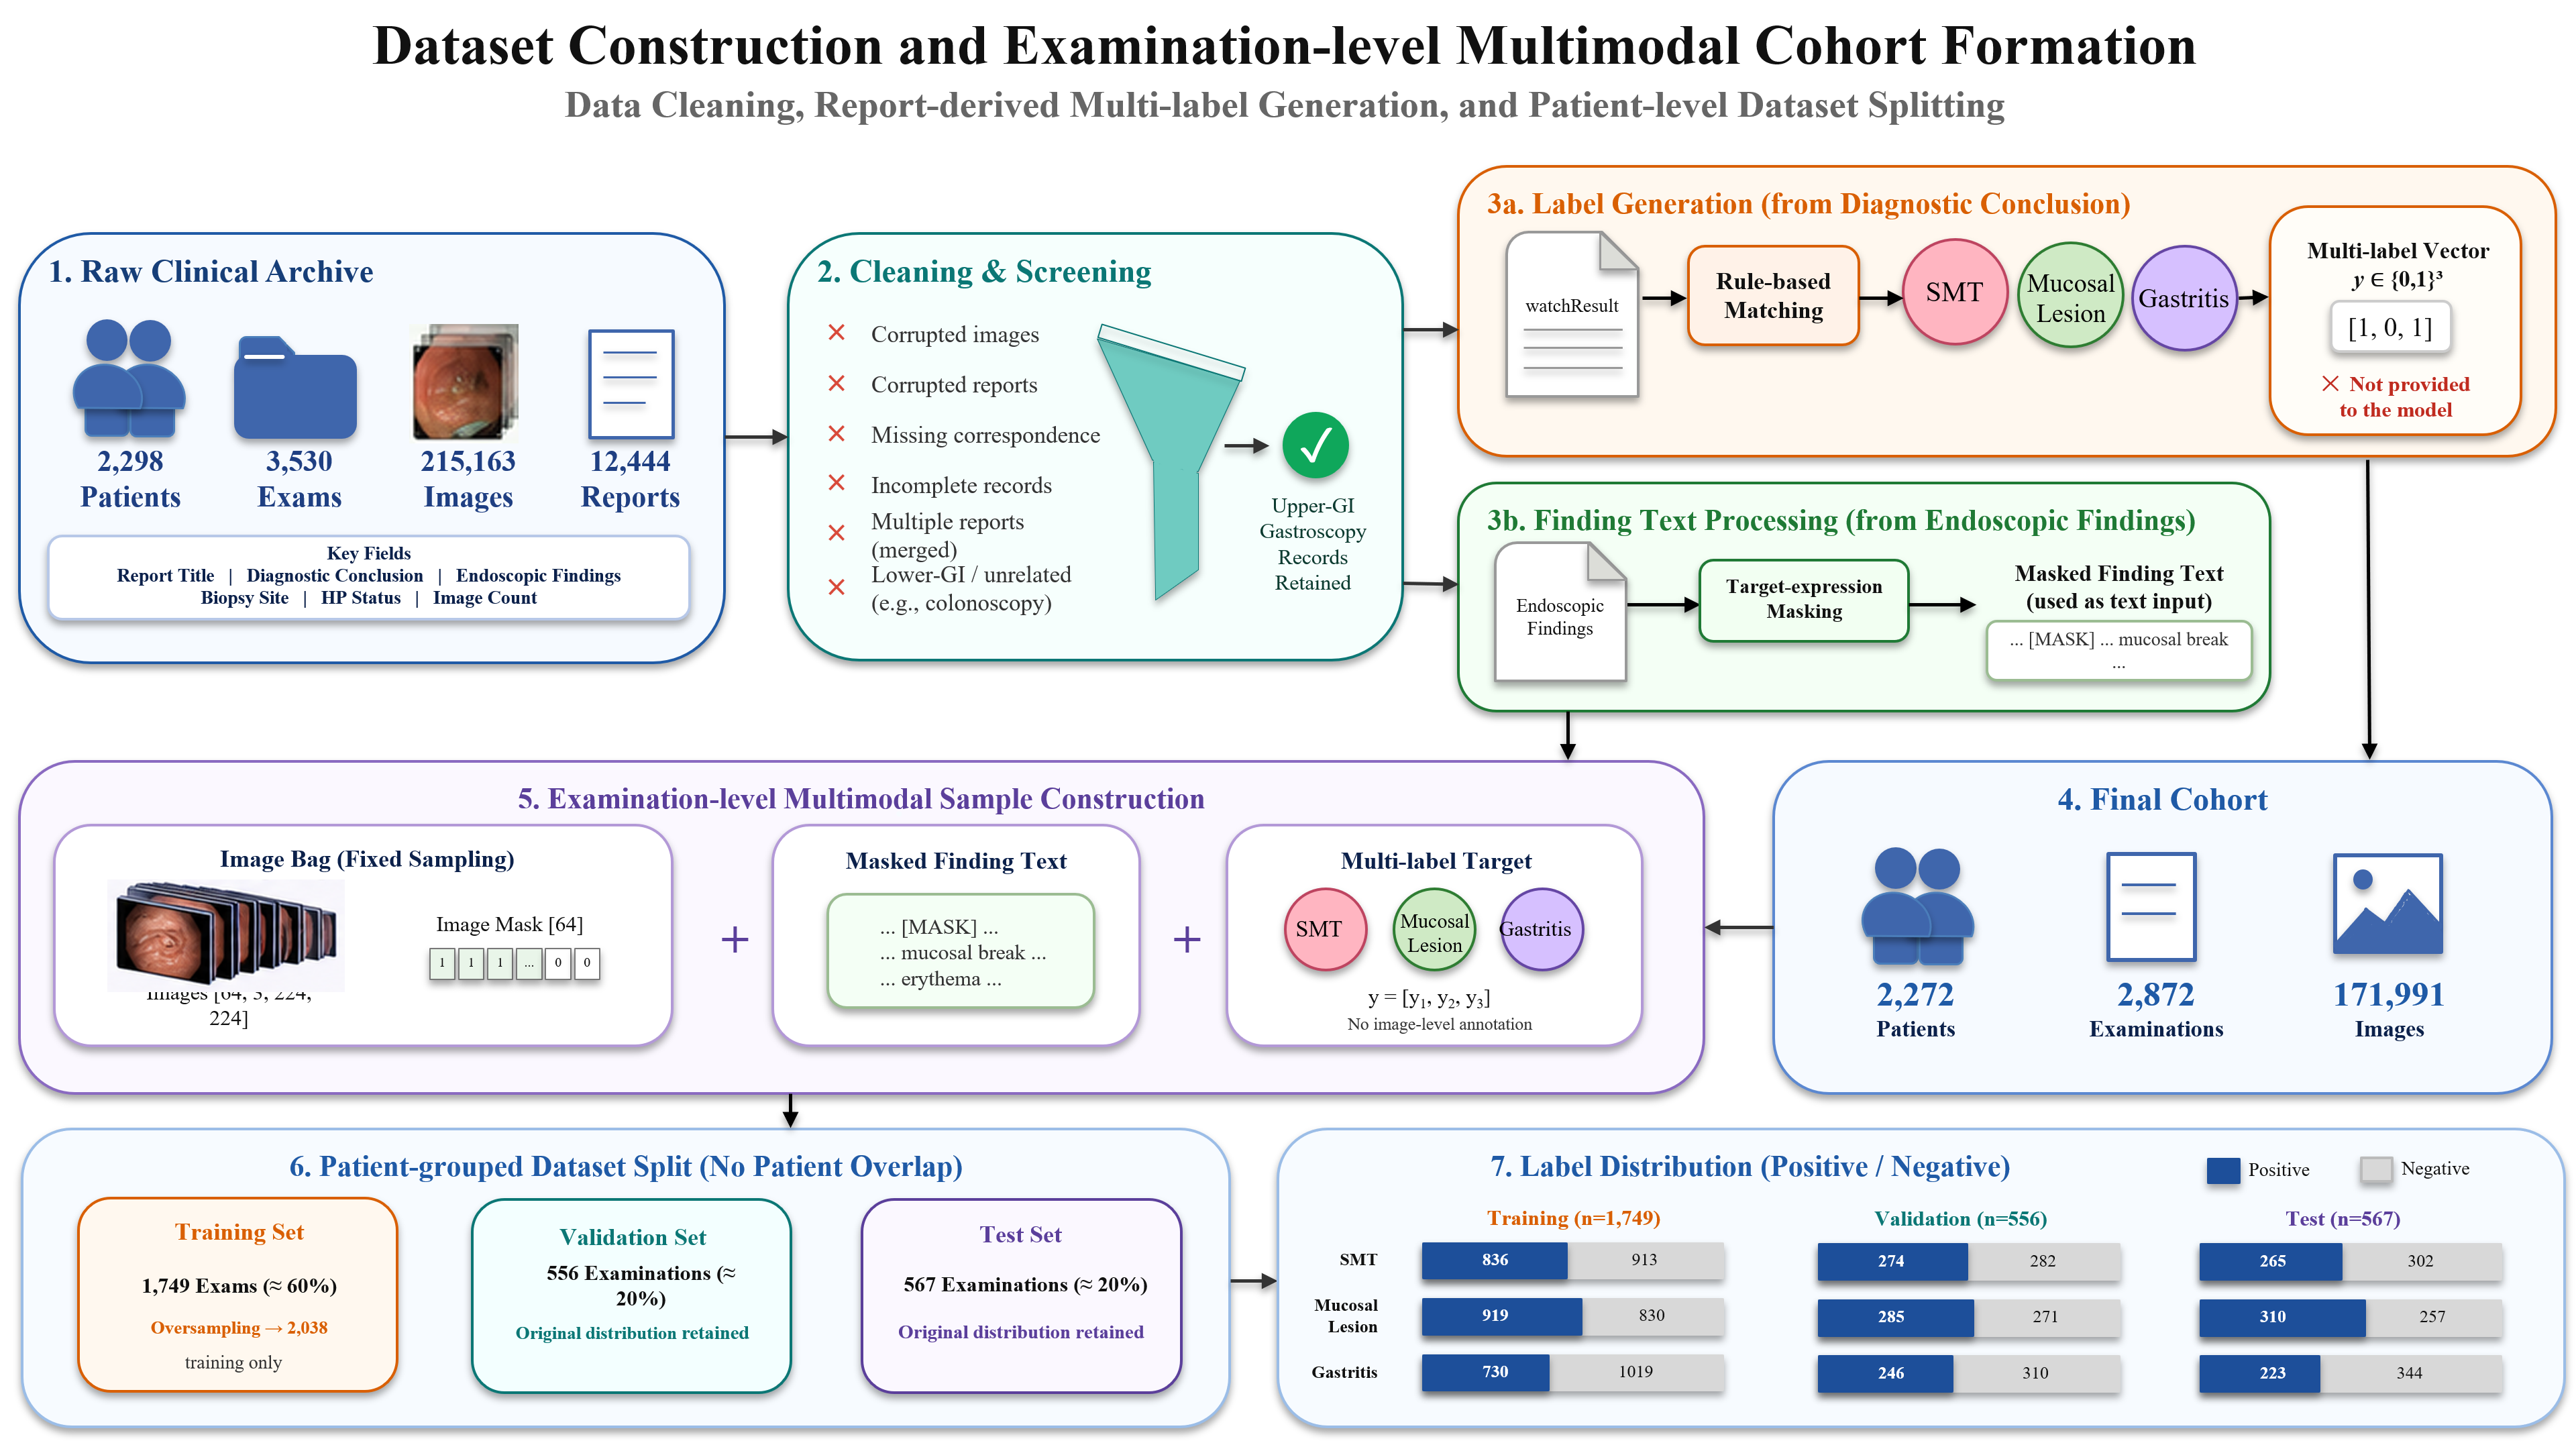
\includegraphics[width=\textwidth]{figs/dataset_construction_pipeline.png}
\caption{Dataset construction and preprocessing pipeline. Raw image--report records were cleaned and standardized, examination-level labels were derived from diagnostic conclusions, direct target expressions were masked in the endoscopic finding text, and patient-grouped subsets were prepared for multimodal learning.\label{fig:dataset_pipeline}}
\end{figure*}

\subsubsection{Data cleaning, standardization, and screening}

Before constructing the task samples, we first performed data cleaning on the raw archive. The raw dataset contained 2298 patients, 3530 examination directories, 215163 images, and 12444 examination reports. Examination records with corrupted images, corrupted reports, or incomplete image-report correspondence were removed. When multiple reports were available for the same examination, the relevant report contents were merged. This step excluded incomplete records and established a reliable basis for subsequent standardization, screening, label derivation, and model training.

\textbf{中文翻译：} 在构建任务样本前，我们首先对原始归档数据进行清洗。原始数据共包含2298名患者、3530个检查目录、215163张图像和12444份检查报告。存在损坏图像、损坏报告或图像与报告对应关系不完整的检查记录被删除；同一次检查存在多份报告时，对相关报告内容进行合并。该步骤用于排除信息不完整的记录，并为后续数据标准化、筛选、标签生成和模型训练建立可靠的数据基础。

After data cleaning, the retained data were standardized into examination-level structured records. Each examination was treated as one independent record, and fields including report title, diagnostic conclusion, endoscopic findings, biopsy site, Helicobacter pylori status, and image count were formatted consistently. Candidate records were screened using the normalized report title and diagnostic conclusion. Records containing upper gastrointestinal terms and no colonoscopy-related terms were retained. This process excluded lower gastrointestinal examinations and retained routine white-light gastroscopy, chromoendoscopy, surgical gastroscopy, endoscopic ultrasound, and related upper gastrointestinal examinations.

\textbf{中文翻译：} 完成数据清洗后，我们将保留数据标准化为检查级结构化记录。每次检查作为一条独立记录，并统一格式化报告标题、诊断结论、内镜所见、活检部位、幽门螺杆菌状态和图像数量等字段。随后，使用规范化后的报告标题和诊断结论筛选候选记录。包含上消化道相关词且不包含肠镜相关词的记录被保留。该过程排除了下消化道检查，并保留常规白光胃镜、染色胃镜、手术胃镜、超声胃镜及相关上消化道检查。

\subsubsection{Report-derived target labels}

Examination-level labels were derived only from the diagnostic conclusions written by physicians. Rule-based text matching identified three non-mutually-exclusive target categories. The esophageal submucosal tumor label matched expressions related to esophageal submucosal tumor, submucosal elevation, and protruding lesion. The esophageal mucosal lesion label matched expressions related to esophageal mucosal lesion, esophageal mass, occupation, and neoplasm. The gastritis label matched chronic, active, inactive, atrophic, erosive, superficial, and bile reflux gastritis, as well as Kimura--Takemoto atrophy grades C1--O3. Esophageal mucosal lesion was treated as an operational report-derived category covering visible or suspicious mucosal abnormalities rather than as a single histopathological entity.

\textbf{中文翻译：} 检查级标签仅由医生书写的诊断结论生成。本文通过规则匹配识别三个互不排斥的目标类别。食管黏膜下肿瘤标签匹配食管黏膜下肿瘤、黏膜下隆起和隆起性病变等相关表述；食管粘膜病变标签匹配食管粘膜病变、食管肿物、食管占位和食管新生物等相关表述；胃炎标签匹配慢性、活动性、非活动性、萎缩性、糜烂性、浅表性和胆汁反流性胃炎，以及Kimura--Takemoto分型中的C1--O3萎缩分级。本文将食管粘膜病变视为覆盖可见或可疑粘膜异常的报告派生操作性类别，而不是单一组织病理学实体。

Records were excluded when the diagnostic conclusion was empty, no target label was matched, or only uncertain descriptions were present without satisfying the matching rules. Examinations matching at least one target label were retained, including those with coexisting findings. The physician-written diagnostic conclusions were used only to construct the target vector and were not used as model input during training, validation, or testing.

\textbf{中文翻译：} 诊断结论为空、未匹配任何目标标签，或仅包含不确定性描述但不满足匹配规则的记录被排除。凡命中至少一个目标标签的检查均被保留，包括存在多个共存发现的检查。医生书写的诊断结论仅用于构建目标向量，在训练、验证和测试阶段均不作为模型输入。

After cleaning, gastroscopy screening, and label generation, the final cohort contained 2872 examinations from 2272 patients and 171991 images. The examinations were divided into training, validation, and test sets with patient grouping at an approximate ratio of 6:2:2. The resulting subsets contained 1749, 556, and 567 examinations, respectively. Patient grouping ensured that examinations from the same patient did not appear in different subsets. Multilabel minority oversampling was applied only to the training set, increasing the effective training exposures from 1749 to 2038; validation and test distributions were unchanged.

\textbf{中文翻译：} 经过数据清洗、胃镜筛选和标签生成后，最终队列包含来自2272名患者的2872次检查和171991张图像。所有检查按患者分组，并以约6:2:2的比例划分为训练集、验证集和测试集，分别包含1749、556和567次检查。患者分组保证同一患者的不同检查不会出现在不同子集中。多标签少数类别过采样仅用于训练集，使有效训练曝光数从1749增加至2038；验证集和测试集分布保持不变。

\begin{table*}[h]
\small\sf\centering
\caption{Label distribution in the training, validation, and test sets.\label{T1}}
\begin{tabular}{lrrrrrr}
\toprule
Label & \multicolumn{2}{c}{\shortstack{Training\\(n=1749)}} & \multicolumn{2}{c}{\shortstack{Validation\\(n=556)}} & \multicolumn{2}{c}{\shortstack{Test\\(n=567)}} \\
\cmidrule(lr){2-3}\cmidrule(lr){4-5}\cmidrule(lr){6-7}
 & Positive & Negative & Positive & Negative & Positive & Negative \\
\midrule
Esophageal submucosal tumor & 836 & 913 & 274 & 282 & 265 & 302 \\
Esophageal mucosal lesion & 919 & 830 & 285 & 271 & 310 & 257 \\
Gastritis & 730 & 1019 & 246 & 310 & 223 & 344 \\
\bottomrule
\end{tabular}
\end{table*}

The label co-occurrence matrix in Figure~\ref{fig:label_cooccurrence} summarizes the multi-label structure of the complete cohort. Gastritis frequently co-occurred with both esophageal targets, whereas direct co-occurrence between the two esophageal labels was less common. This pattern motivated explicit modeling of higher-order label relationships.

\textbf{中文翻译：} 图~\ref{fig:label_cooccurrence}展示了完整队列的标签共现结构。胃炎与两个食管标签均存在较多共现，而两个食管标签之间的直接共现相对较少，这一分布为显式建模高阶标签关系提供了依据。

\begin{figure*}[t]
\centering
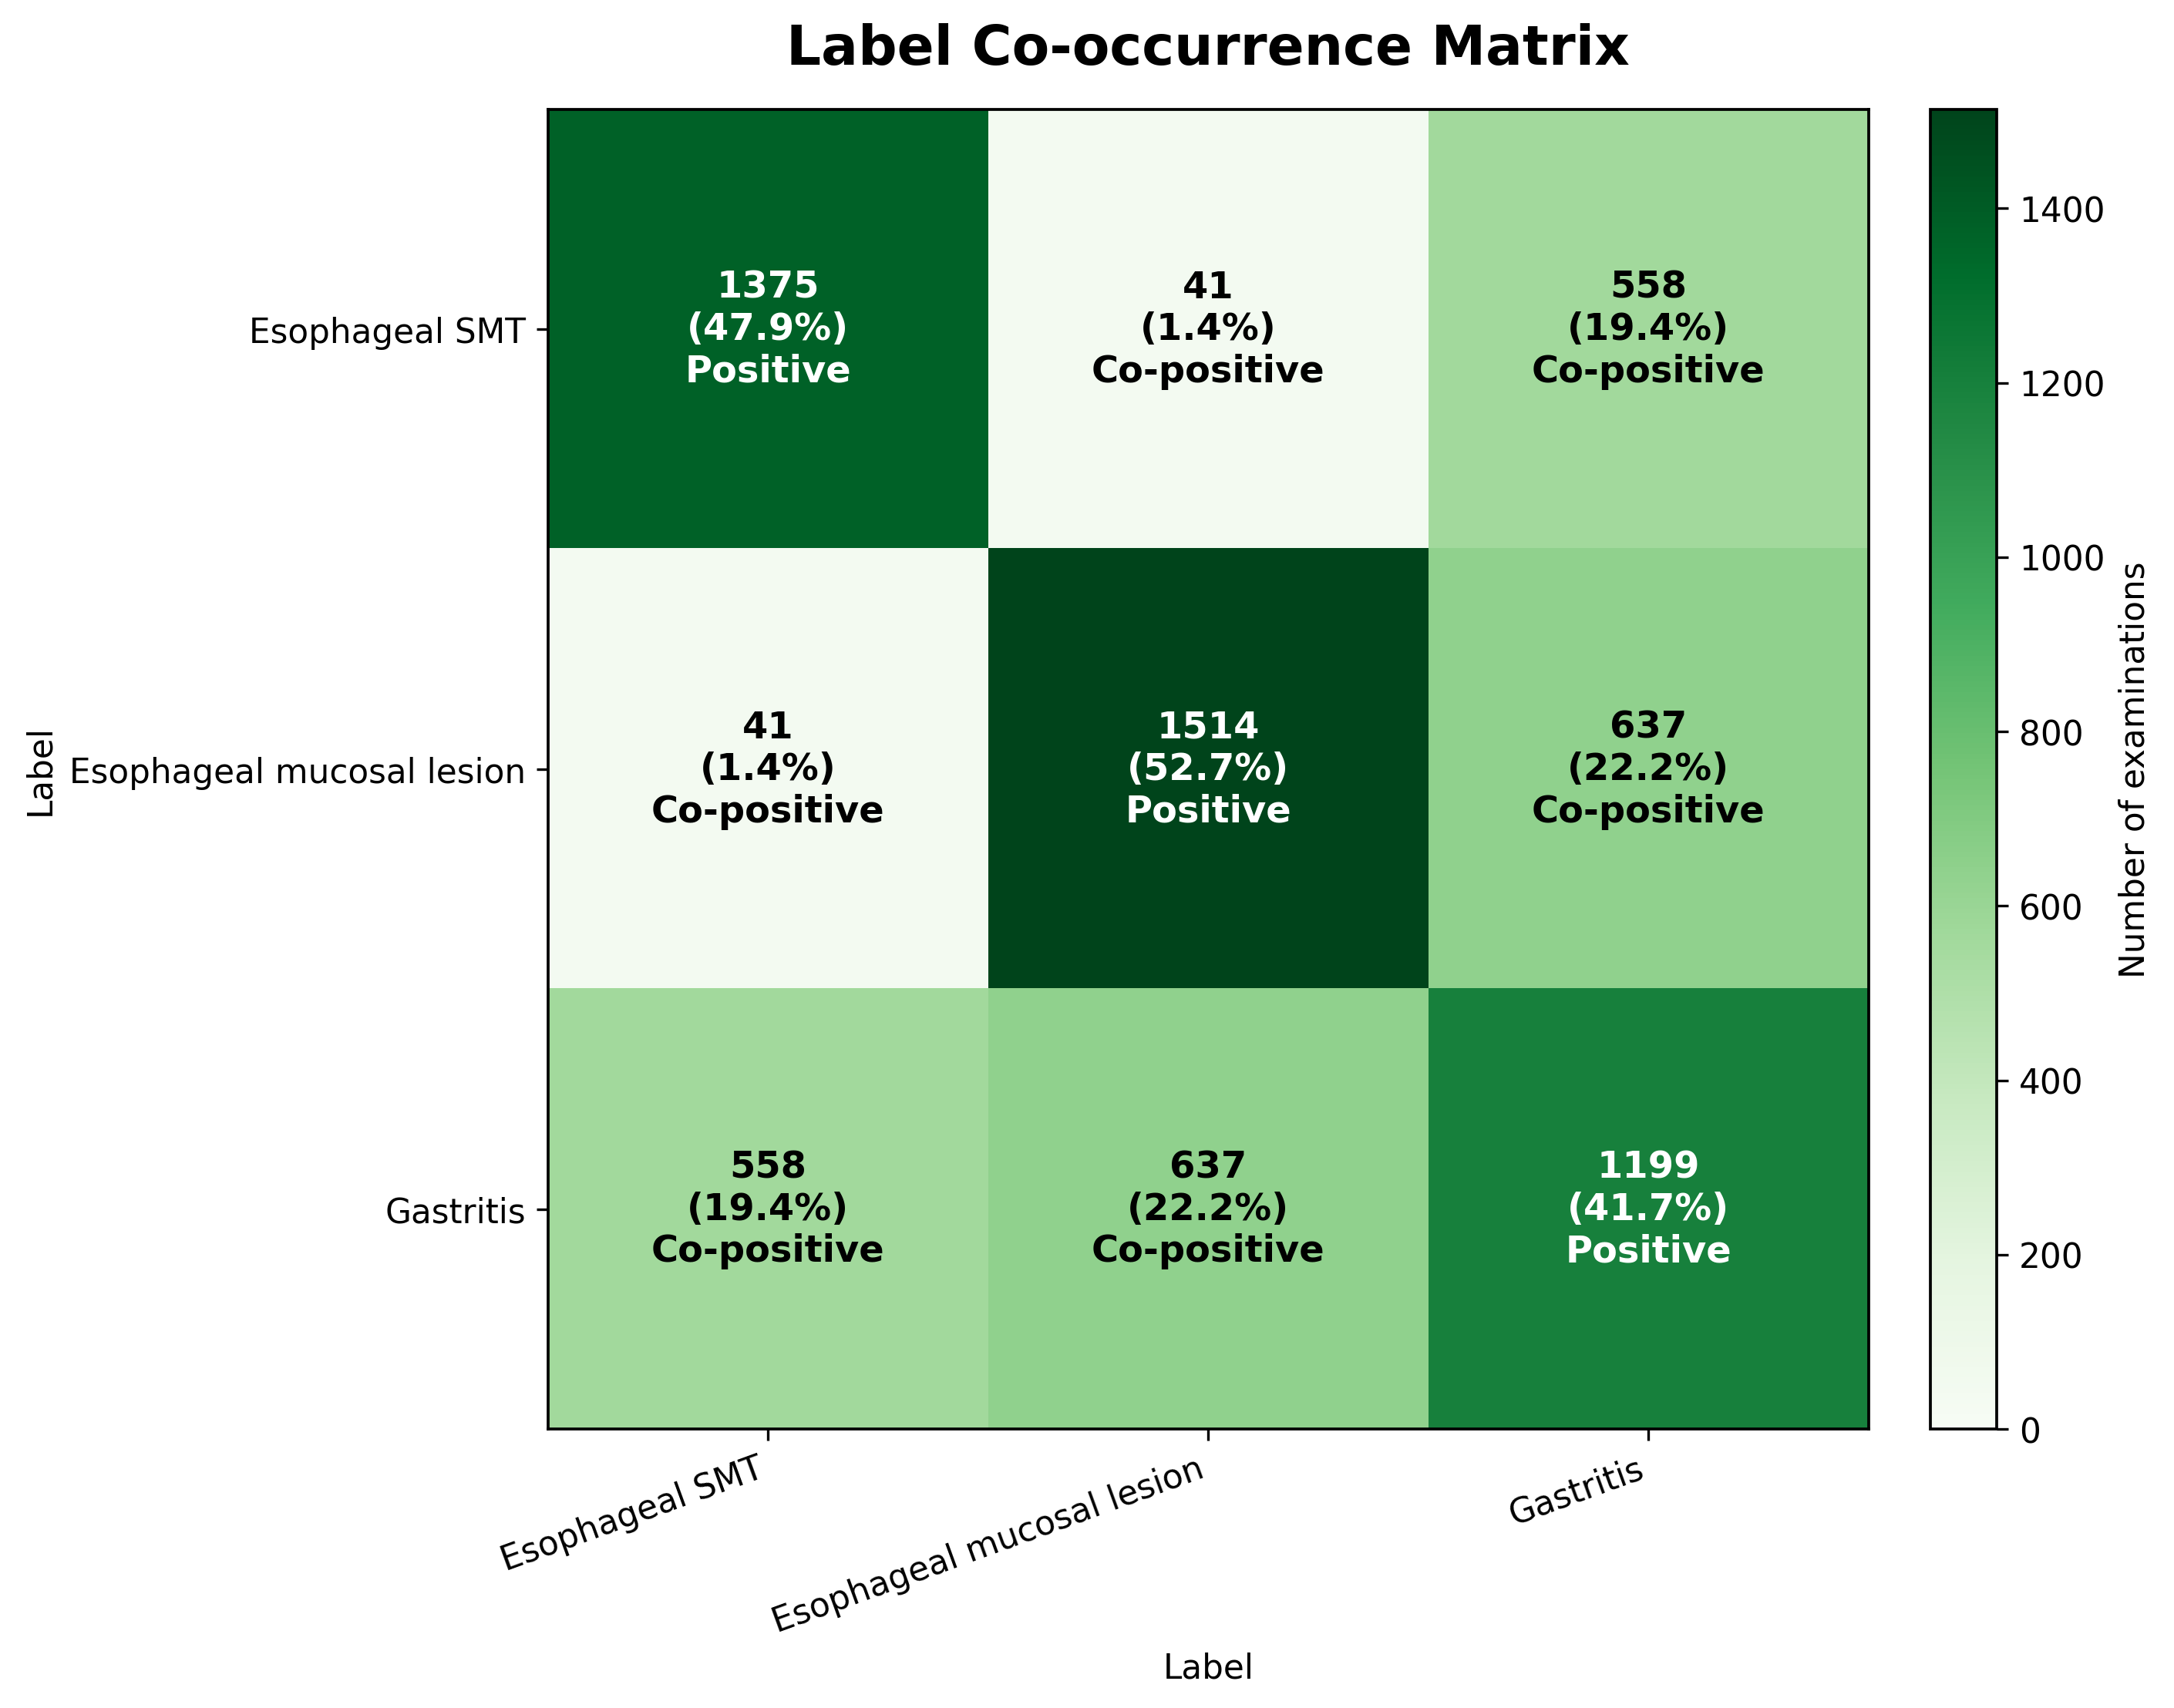
\includegraphics[width=0.72\textwidth]{figs/label_cooccurrence_matrix.png}
\caption{Label co-occurrence matrix for all 2872 examinations. Diagonal cells show the number of positive examinations for each label, and off-diagonal cells show the number of examinations in which the corresponding label pair co-occurred; percentages are relative to the full cohort.\label{fig:label_cooccurrence}}
\end{figure*}

\subsubsection{Examination-level multimodal sample construction}

Each eligible examination was represented by its complete ordered image sequence, a three-dimensional multi-label target, and the physician-written endoscopic finding narrative. For model preparation, at most $T=64$ images were uniformly sampled from each examination while preserving their original order. Each image was resized to 224$\times$224 pixels. A binary mask $M_i=\{m_{i1},\ldots,m_{iT}\}$ distinguished valid images from padded positions. The matched endoscopic finding narrative was retained as the report input; its category masking and encoding procedures are described in the text branch. The overall MEF-CAH-MIL architecture is shown in Figure~\ref{fig:model_architecture}.

\textbf{中文翻译：} 每次符合条件的检查由完整有序图像序列、三维多标签目标和医生书写的内镜所见文本表示。模型准备阶段从每次检查中最多均匀采样$T=64$张图像，并保持其原始顺序。每张图像被缩放至224$\times$224像素。二值掩码$M_i=\{m_{i1},\ldots,m_{iT}\}$用于区分有效图像和填充位置。与检查匹配的内镜所见文本作为报告输入，其类别掩码和编码过程将在文本分支中说明。MEF-CAH-MIL的整体结构如图~\ref{fig:model_architecture}所示。

\begin{figure*}[t]
\centering
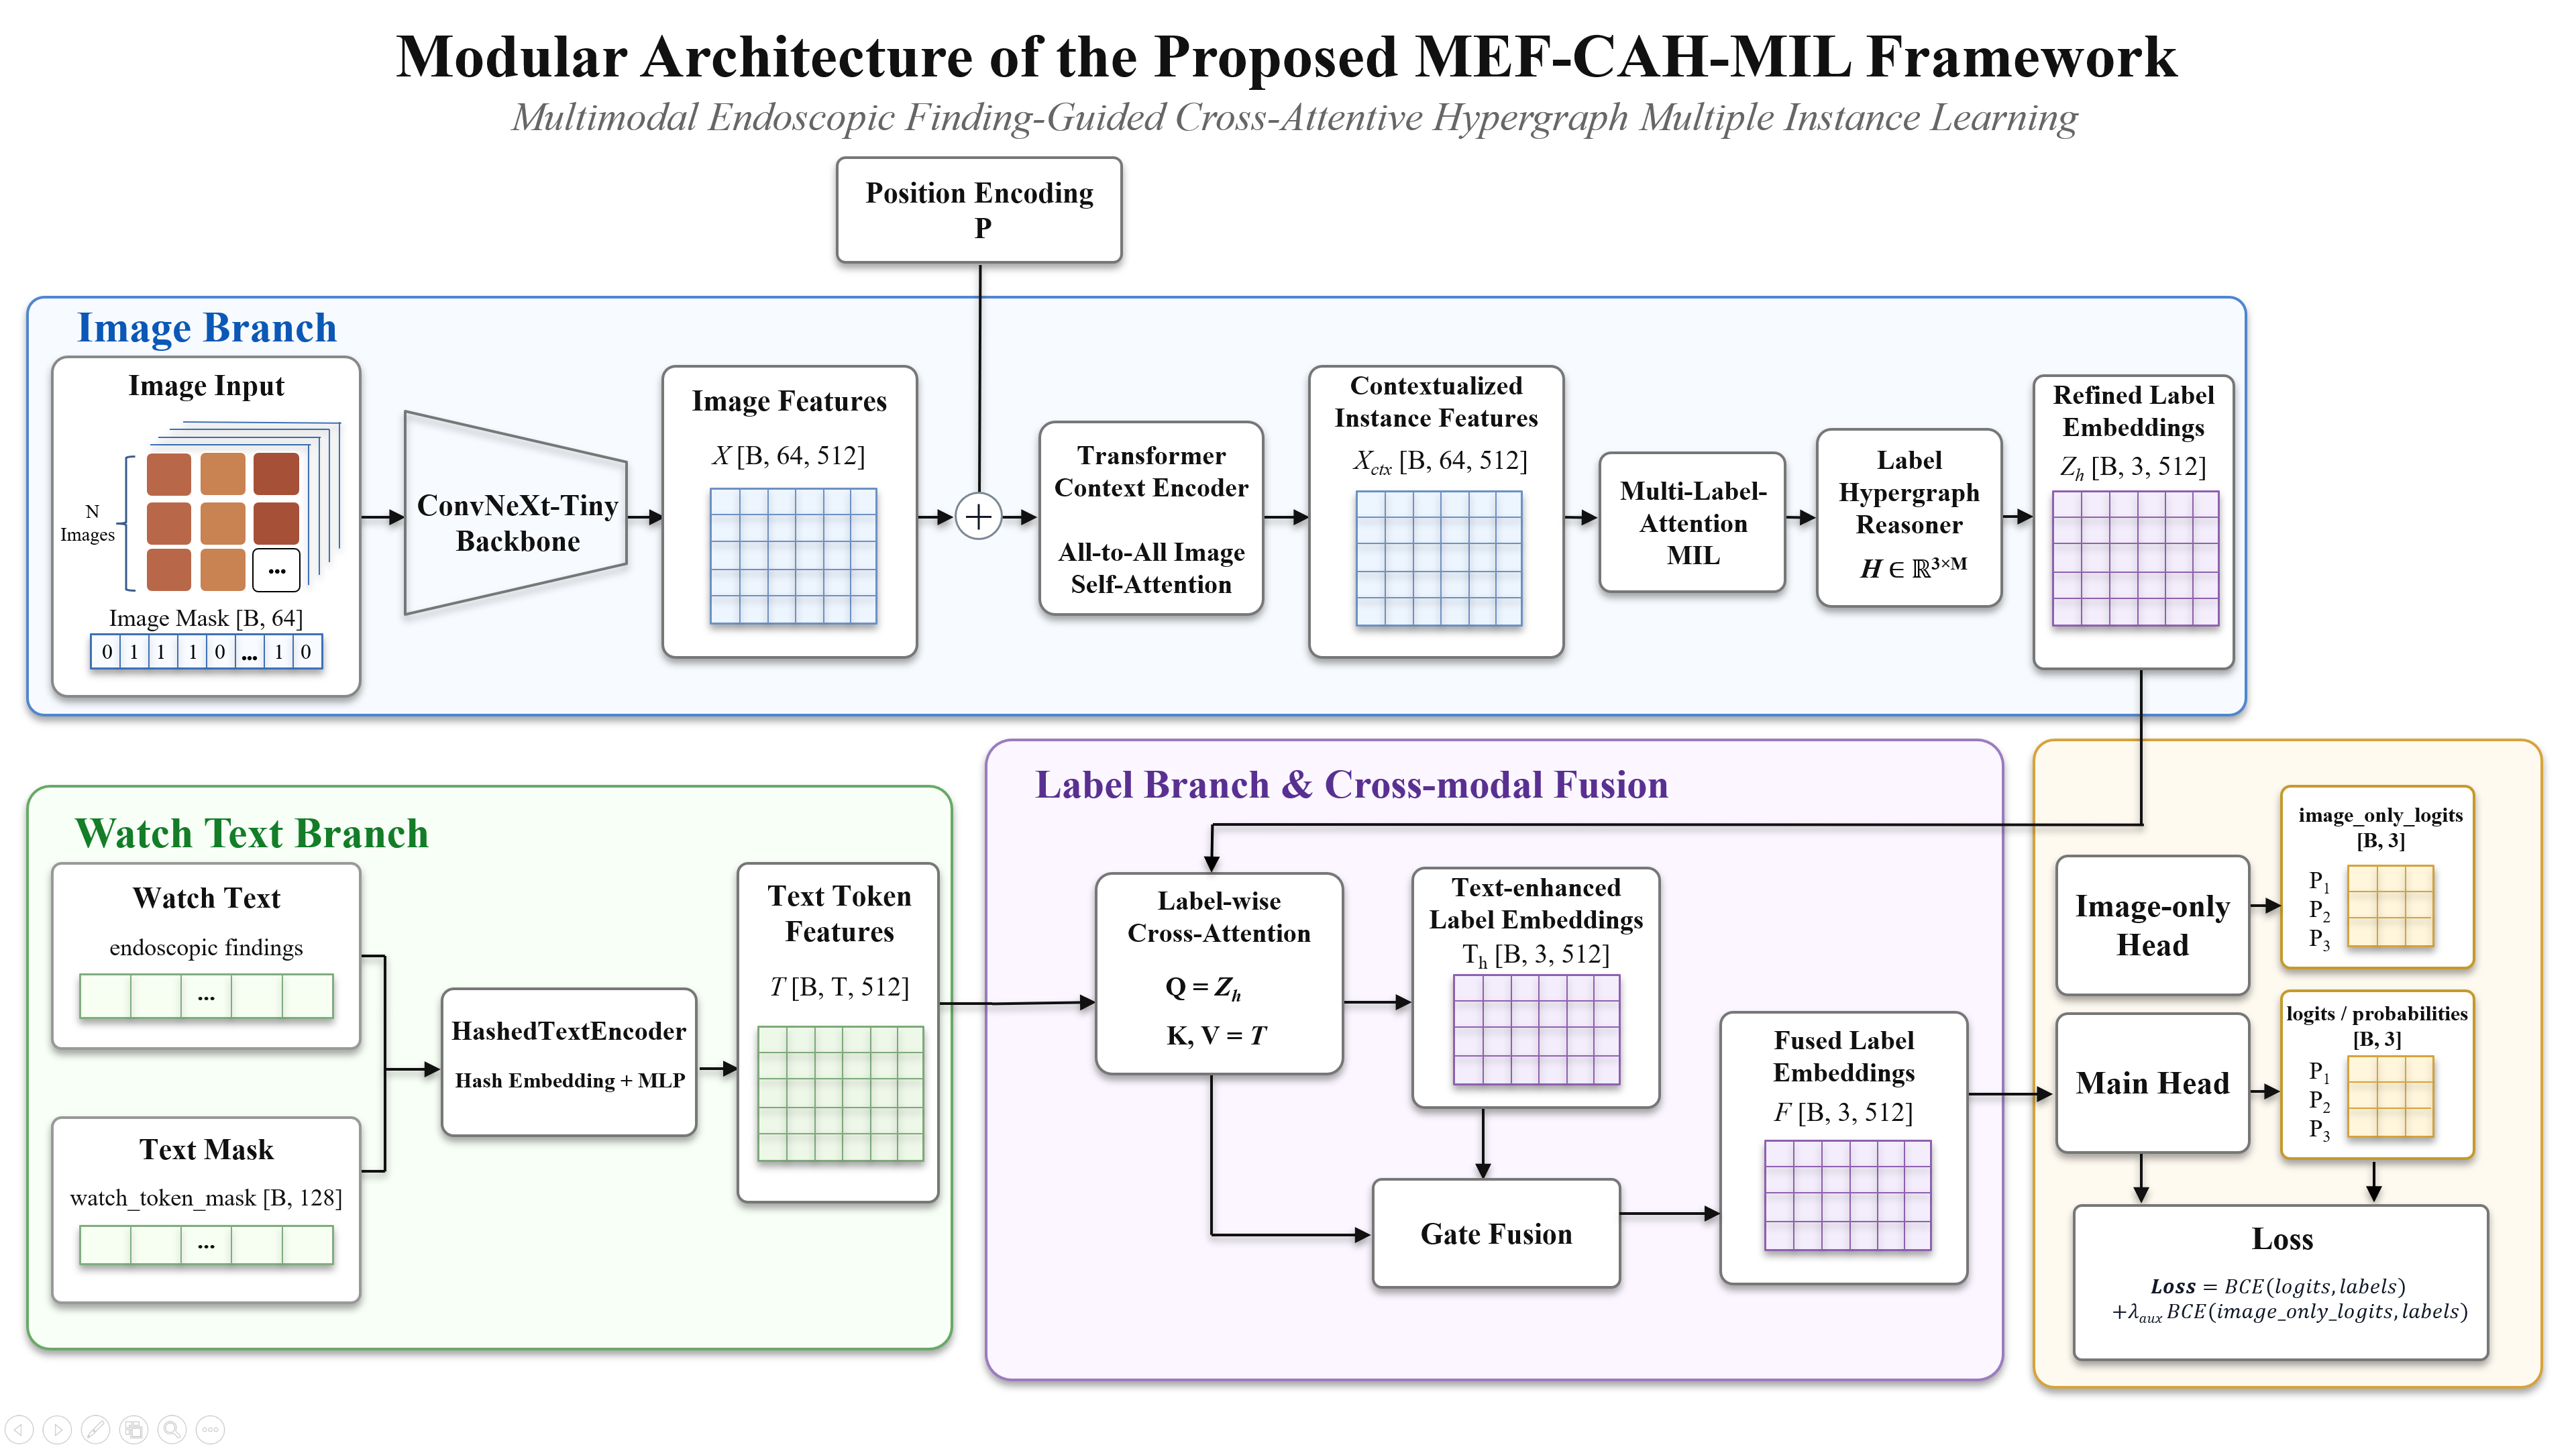
\includegraphics[width=\textwidth]{figs/mef_cah_mil_architecture.png}
\caption{Overall architecture of MEF-CAH-MIL. The image branch models ordered endoscopic images and label relations, the text branch encodes category-masked endoscopic findings, and label-query cross-attention with gated fusion produces the multimodal prediction.\label{fig:model_architecture}}
\end{figure*}

\subsection{Image Branch}

For the $i$-th gastroscopy examination, let $X_i=\{I_{i1},I_{i2},\ldots,I_{iN_i}\}$ denote its variable-length image bag, $M_i$ the valid-image mask, and $y_i\in\{0,1\}^{L}$ the examination-level target, where $L=3$. The three dimensions correspond to esophageal submucosal tumor, esophageal mucosal lesion, and gastritis, and more than one label may be positive in the same examination. The image branch maps $X_i$ and $M_i$ to label-specific visual representations and an image-only prediction $p_i^{img}=G_{\Theta}(X_i,M_i)$.

\textbf{中文翻译：} 对于第$i$次胃镜检查，令$X_i=\{I_{i1},I_{i2},\ldots,I_{iN_i}\}$表示变长图像bag，$M_i$表示有效图像掩码，$y_i\in\{0,1\}^{L}$表示检查级目标，其中$L=3$。三个维度分别对应食管黏膜下肿瘤、食管粘膜病变和胃炎，同一次检查可以同时具有多个阳性标签。图像分支根据$X_i$和$M_i$生成标签特异性视觉表征及纯图像预测$p_i^{img}=G_{\Theta}(X_i,M_i)$。

\subsubsection{Image encoding and position-aware context modeling}

Each sampled image was encoded by a shared ConvNeXt-Tiny backbone followed by a projection head, producing a $d=512$ dimensional instance feature.\cite{R11} To retain sequence information, a position encoding was added to the image features before they were passed through a two-layer Transformer encoder with four attention heads:\cite{R13}
\begin{equation}
H_i=\mathrm{Transformer}\left(f_{\theta}(X_i)+P_i,M_i\right),
\end{equation}
where $H_i=\{h_{i1},\ldots,h_{iT}\}\in\mathbb{R}^{T\times d}$ contains the contextualized image features. The valid-image mask was used throughout the Transformer to exclude padded positions. Figure~\ref{fig:position_context} summarizes the position and intra-examination context encoding process.

\textbf{中文翻译：} 每张采样图像由共享的ConvNeXt-Tiny骨干网络和投影头进行编码，得到$d=512$维实例特征。为保留序列信息，图像特征加入位置编码后输入包含两层和四个注意力头的Transformer编码器：
\begin{equation}
H_i=\mathrm{Transformer}\left(f_{\theta}(X_i)+P_i,M_i\right),
\end{equation}
其中$H_i=\{h_{i1},\ldots,h_{iT}\}\in\mathbb{R}^{T\times d}$表示上下文化后的图像特征。Transformer在整个计算过程中使用有效图像掩码排除填充位置。图~\ref{fig:position_context}概括了该模块对位置和检查内上下文的编码过程。

\begin{figure*}[t]
\centering
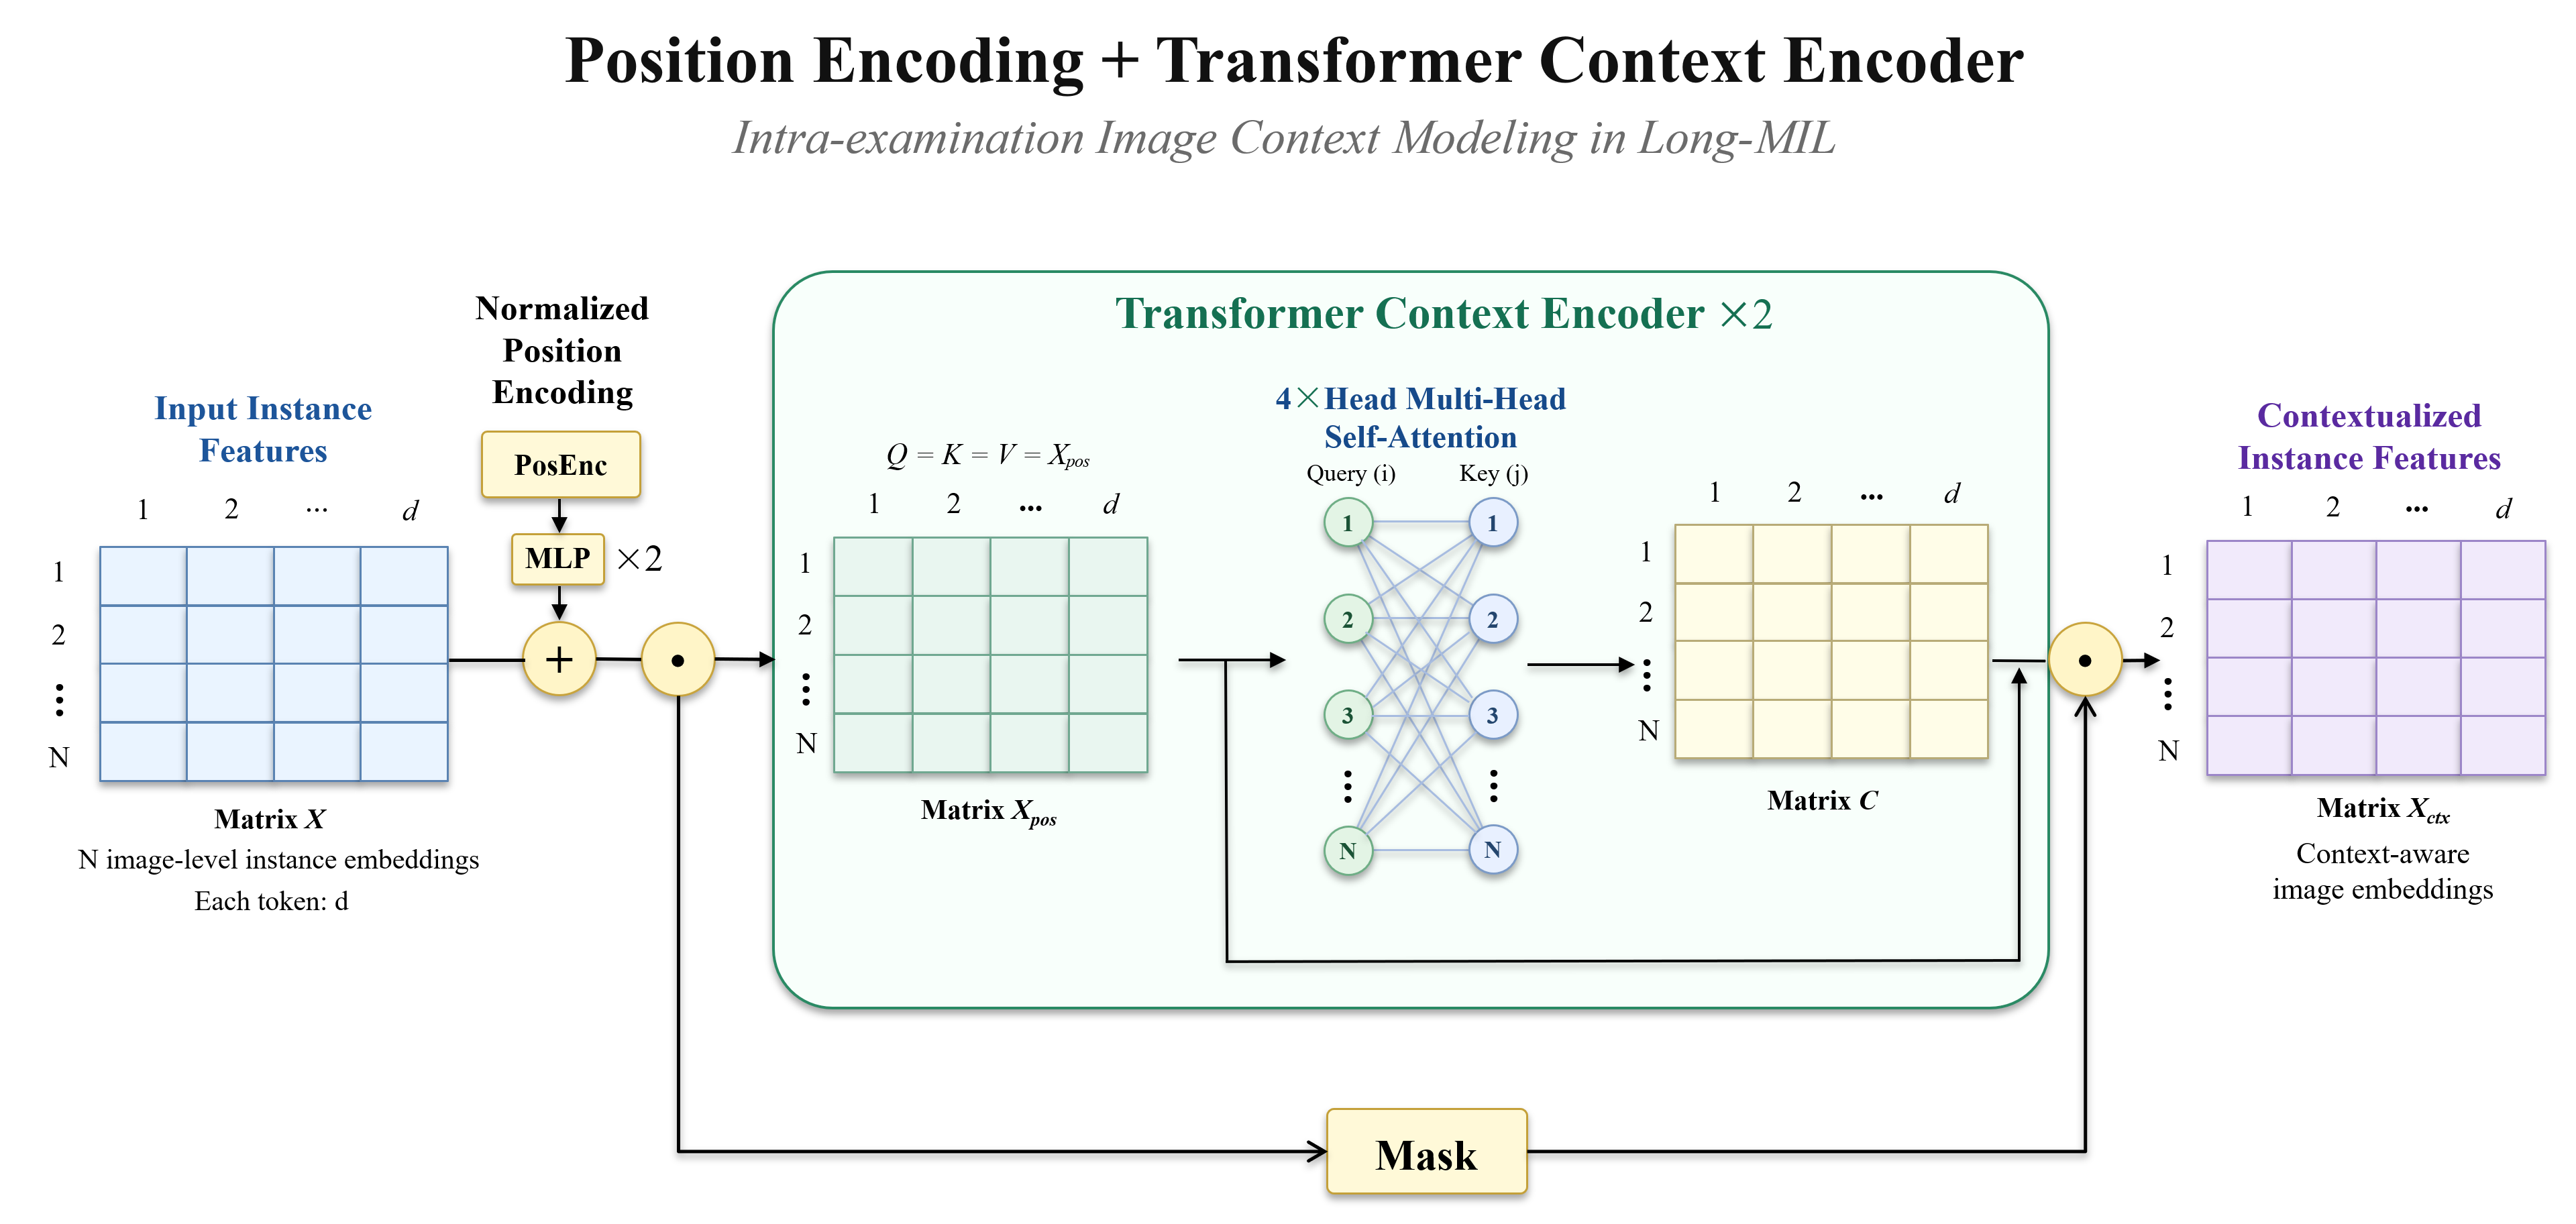
\includegraphics[width=\textwidth]{figs/position_context_encoder.png}
\caption{Position-aware intra-examination context encoder. Projected image features are augmented with positional information and contextualized by a two-layer, four-head Transformer while padded positions are excluded by the valid-image mask.\label{fig:position_context}}
\end{figure*}

\subsubsection{Multi-label attention MIL}

Different diseases may be supported by different images in the same examination. The model therefore learned one gated attention distribution for each label. For image $n$, the shared gated attention feature was
\begin{equation}
q_{in}=\tanh(Vh_{in})\odot\sigma(Uh_{in}),
\end{equation}
and the normalized attention weight for label $\ell$ was
\begin{equation}
a_{i\ell n}=\frac{m_{in}\exp(w_{\ell}^{\top}q_{in})}{\sum_{t=1}^{T}m_{it}\exp(w_{\ell}^{\top}q_{it})+\epsilon}.
\end{equation}
The label-specific visual representation was obtained as
\begin{equation}
z_{i\ell}=\sum_{n=1}^{T}a_{i\ell n}h_{in}.
\end{equation}
This operation allows each disease to aggregate its own supporting images while ignoring invalid positions.

\textbf{中文翻译：} 同一次检查中的不同疾病可能由不同图像提供证据，因此模型为每个标签分别学习门控注意力分布。对于图像$n$，共享门控注意力特征为
\begin{equation}
q_{in}=\tanh(Vh_{in})\odot\sigma(Uh_{in}),
\end{equation}
标签$\ell$对应的归一化注意力权重为
\begin{equation}
a_{i\ell n}=\frac{m_{in}\exp(w_{\ell}^{\top}q_{in})}{\sum_{t=1}^{T}m_{it}\exp(w_{\ell}^{\top}q_{it})+\epsilon}.
\end{equation}
标签特异性视觉表征计算为
\begin{equation}
z_{i\ell}=\sum_{n=1}^{T}a_{i\ell n}h_{in}.
\end{equation}
该操作使每种疾病能够聚合各自的支持图像，同时忽略无效位置。

\subsubsection{Label hypergraph reasoning and image-only prediction}

Let $Z_i=[z_{i1},\ldots,z_{iL}]^{\top}\in\mathbb{R}^{L\times d}$ denote the label-specific visual feature matrix. To model higher-order relationships among coexisting diseases, the label hypergraph reasoner learned an incidence matrix $B\in\mathbb{R}^{L\times E}$ with $E=2$ latent hyperedges. After normalization, information was propagated from label nodes to hyperedges and then back to label nodes:
\begin{equation}
U_i=S_{node\rightarrow edge}^{\top}\eta(Z_i),
\end{equation}
\begin{equation}
\widetilde{Z}_i=S_{edge\rightarrow node}U_i,
\end{equation}
\begin{equation}
Z_i^{img}=Z_i+\phi([Z_i;\widetilde{Z}_i]),
\end{equation}
where $\eta(\cdot)$ and $\phi(\cdot)$ are learnable transformations. The image-only logits were produced before text fusion as $s_i^{img}=C(Z_i^{img})$. Figure~\ref{fig:attention_hypergraph} illustrates disease-specific image aggregation followed by label hypergraph reasoning.

\textbf{中文翻译：} 令$Z_i=[z_{i1},\ldots,z_{iL}]^{\top}\in\mathbb{R}^{L\times d}$表示标签特异性视觉特征矩阵。为建模多个共存疾病之间的高阶关系，标签超图推理器学习关联矩阵$B\in\mathbb{R}^{L\times E}$，其中$E=2$表示两个潜在超边。归一化后，信息先从标签节点传播到超边，再从超边返回标签节点：
\begin{equation}
U_i=S_{node\rightarrow edge}^{\top}\eta(Z_i),
\end{equation}
\begin{equation}
\widetilde{Z}_i=S_{edge\rightarrow node}U_i,
\end{equation}
\begin{equation}
Z_i^{img}=Z_i+\phi([Z_i;\widetilde{Z}_i]),
\end{equation}
其中$\eta(\cdot)$和$\phi(\cdot)$为可学习变换。文本融合前，模型通过$s_i^{img}=C(Z_i^{img})$生成纯图像logits。图~\ref{fig:attention_hypergraph}展示了从疾病特异性图像聚合到标签超图推理的过程。

\begin{figure*}[t]
\centering
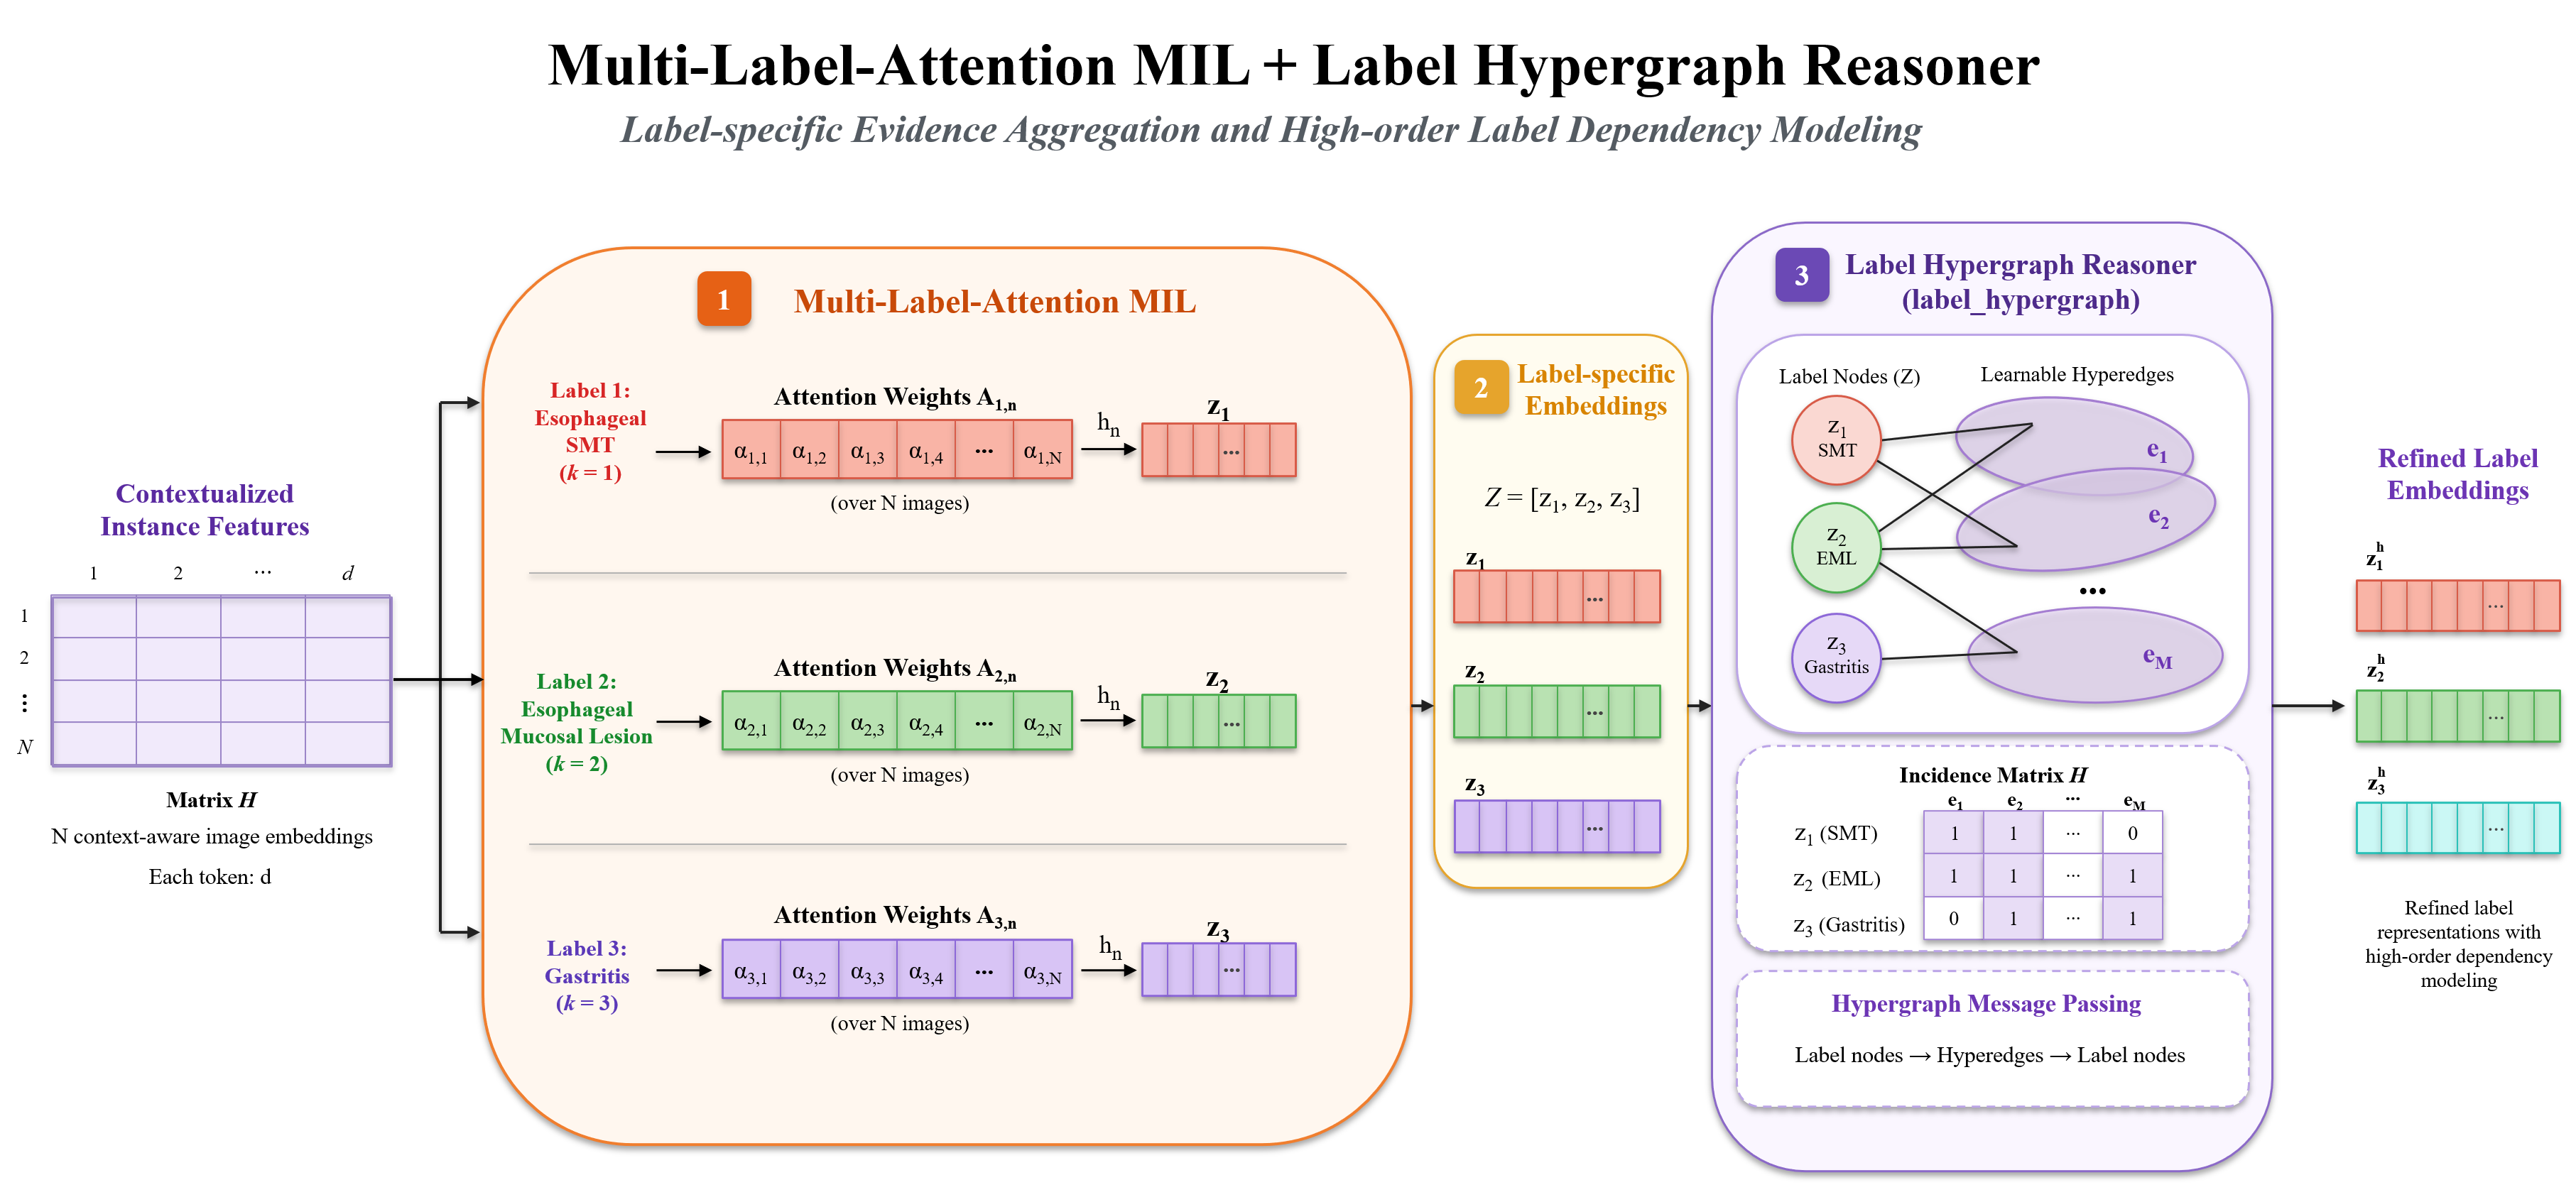
\includegraphics[width=\textwidth]{figs/label_attention_hypergraph_reasoner.png}
\caption{Multi-label attention MIL and label hypergraph reasoning. Label-specific attention aggregates different supporting images for each disease, after which latent hyperedges propagate information among coexisting labels.\label{fig:attention_hypergraph}}
\end{figure*}

\subsection{Text Branch}

\subsubsection{Report field separation and category masking}

The text branch used the physician-written endoscopic finding narrative rather than the diagnostic conclusion used for label derivation. The endoscopic finding narrative describes lesion morphology, location, and surrounding mucosal changes, but it may also directly contain a target category name. To reduce direct label leakage, canonical disease names, abbreviations, and direct lexical variants associated with the three targets were replaced with a common mask token before tokenization. The masking lexicon covered direct category expressions such as esophageal submucosal tumor or SMT, esophageal mucosal lesion, and named forms of gastritis, while retaining anatomical locations and descriptive morphology. The same masking procedure was applied to all data subsets.

\textbf{中文翻译：} 文本分支使用医生书写的内镜所见文本，而不是用于标签生成的诊断结论。内镜所见文本描述病灶形态、位置和周围黏膜改变，但也可能直接包含目标类别名称。为减少直接标签信息泄露，模型在分词前将与三个目标相关的标准疾病名称、缩写和直接词汇变体替换为统一掩码token。掩码词典覆盖食管黏膜下肿瘤或SMT、食管粘膜病变以及不同命名形式的胃炎等直接类别表述，同时保留解剖位置和描述性形态信息。所有数据子集使用相同的掩码过程。

\subsubsection{Hashed text encoding}

After masking, whitespace and punctuation were normalized, and the report was tokenized into Chinese characters and alphanumeric fragments. Each token was mapped by a deterministic hash function to a vocabulary of 8192 indices. A 128-dimensional token embedding was then projected into the same $d=512$ dimensional space as the visual features. The maximum text length was $K=128$, and a text mask excluded padded tokens. The encoded report was written as
\begin{equation}
T_i=\psi_{\omega}(\mathrm{HashTokenize}(W_i))\in\mathbb{R}^{K\times d}.
\end{equation}
This lightweight encoder did not require external language-model weights.

\textbf{中文翻译：} 完成掩码后，文本中的空格和标点被规范化，报告被切分为中文字符和字母数字片段。每个token通过确定性哈希函数映射到大小为8192的词表中，随后将128维token embedding投影到与视觉特征相同的$d=512$维空间。最大文本长度为$K=128$，文本掩码用于排除填充token。编码后的报告表示为
\begin{equation}
T_i=\psi_{\omega}(\mathrm{HashTokenize}(W_i))\in\mathbb{R}^{K\times d}.
\end{equation}
该轻量编码器不依赖外部语言模型权重。

\subsection{Cross-Modal Fusion Branch}

\subsubsection{Label-query cross-attention and gated fusion}

The hypergraph-refined visual representations $Z_i^{img}$ were used as label queries, while the encoded report tokens $T_i$ were used as keys and values. Multi-head cross-attention produced one text representation for each disease label:
\begin{equation}
Z_i^{txt}=\mathrm{CrossAttn}(Q=Z_i^{img},K=T_i,V=T_i).
\end{equation}
This label-query design allows different diseases to retrieve different content from the same report. A label-wise gate then controlled the contribution of the retrieved text:
\begin{equation}
G_i=\sigma\left(\rho([Z_i^{img};Z_i^{txt}])\right),
\end{equation}
\begin{equation}
Z_i^{fuse}=Z_i^{img}+G_i\odot Z_i^{txt},
\end{equation}
where $\rho(\cdot)$ is a multilayer perceptron. When valid report text was absent, the text contribution was set to zero and the fused representation reduced to the visual representation. Figure~\ref{fig:cross_attention_gate} details the cross-attention and gated residual fusion module.

\textbf{中文翻译：} 经过超图推理的视觉表征$Z_i^{img}$作为标签查询，编码后的报告token $T_i$作为key和value。多头cross-attention为每个疾病标签生成一个文本表征：
\begin{equation}
Z_i^{txt}=\mathrm{CrossAttn}(Q=Z_i^{img},K=T_i,V=T_i).
\end{equation}
这种标签查询设计使不同疾病能够从同一份报告中检索不同内容。随后，标签级门控控制所检索文本信息的作用：
\begin{equation}
G_i=\sigma\left(\rho([Z_i^{img};Z_i^{txt}])\right),
\end{equation}
\begin{equation}
Z_i^{fuse}=Z_i^{img}+G_i\odot Z_i^{txt},
\end{equation}
其中$\rho(\cdot)$为多层感知机。当不存在有效报告文本时，文本贡献被设为零，融合表征退化为视觉表征。图~\ref{fig:cross_attention_gate}展示了标签查询cross-attention和门控残差融合的具体结构。

\begin{figure*}[t]
\centering
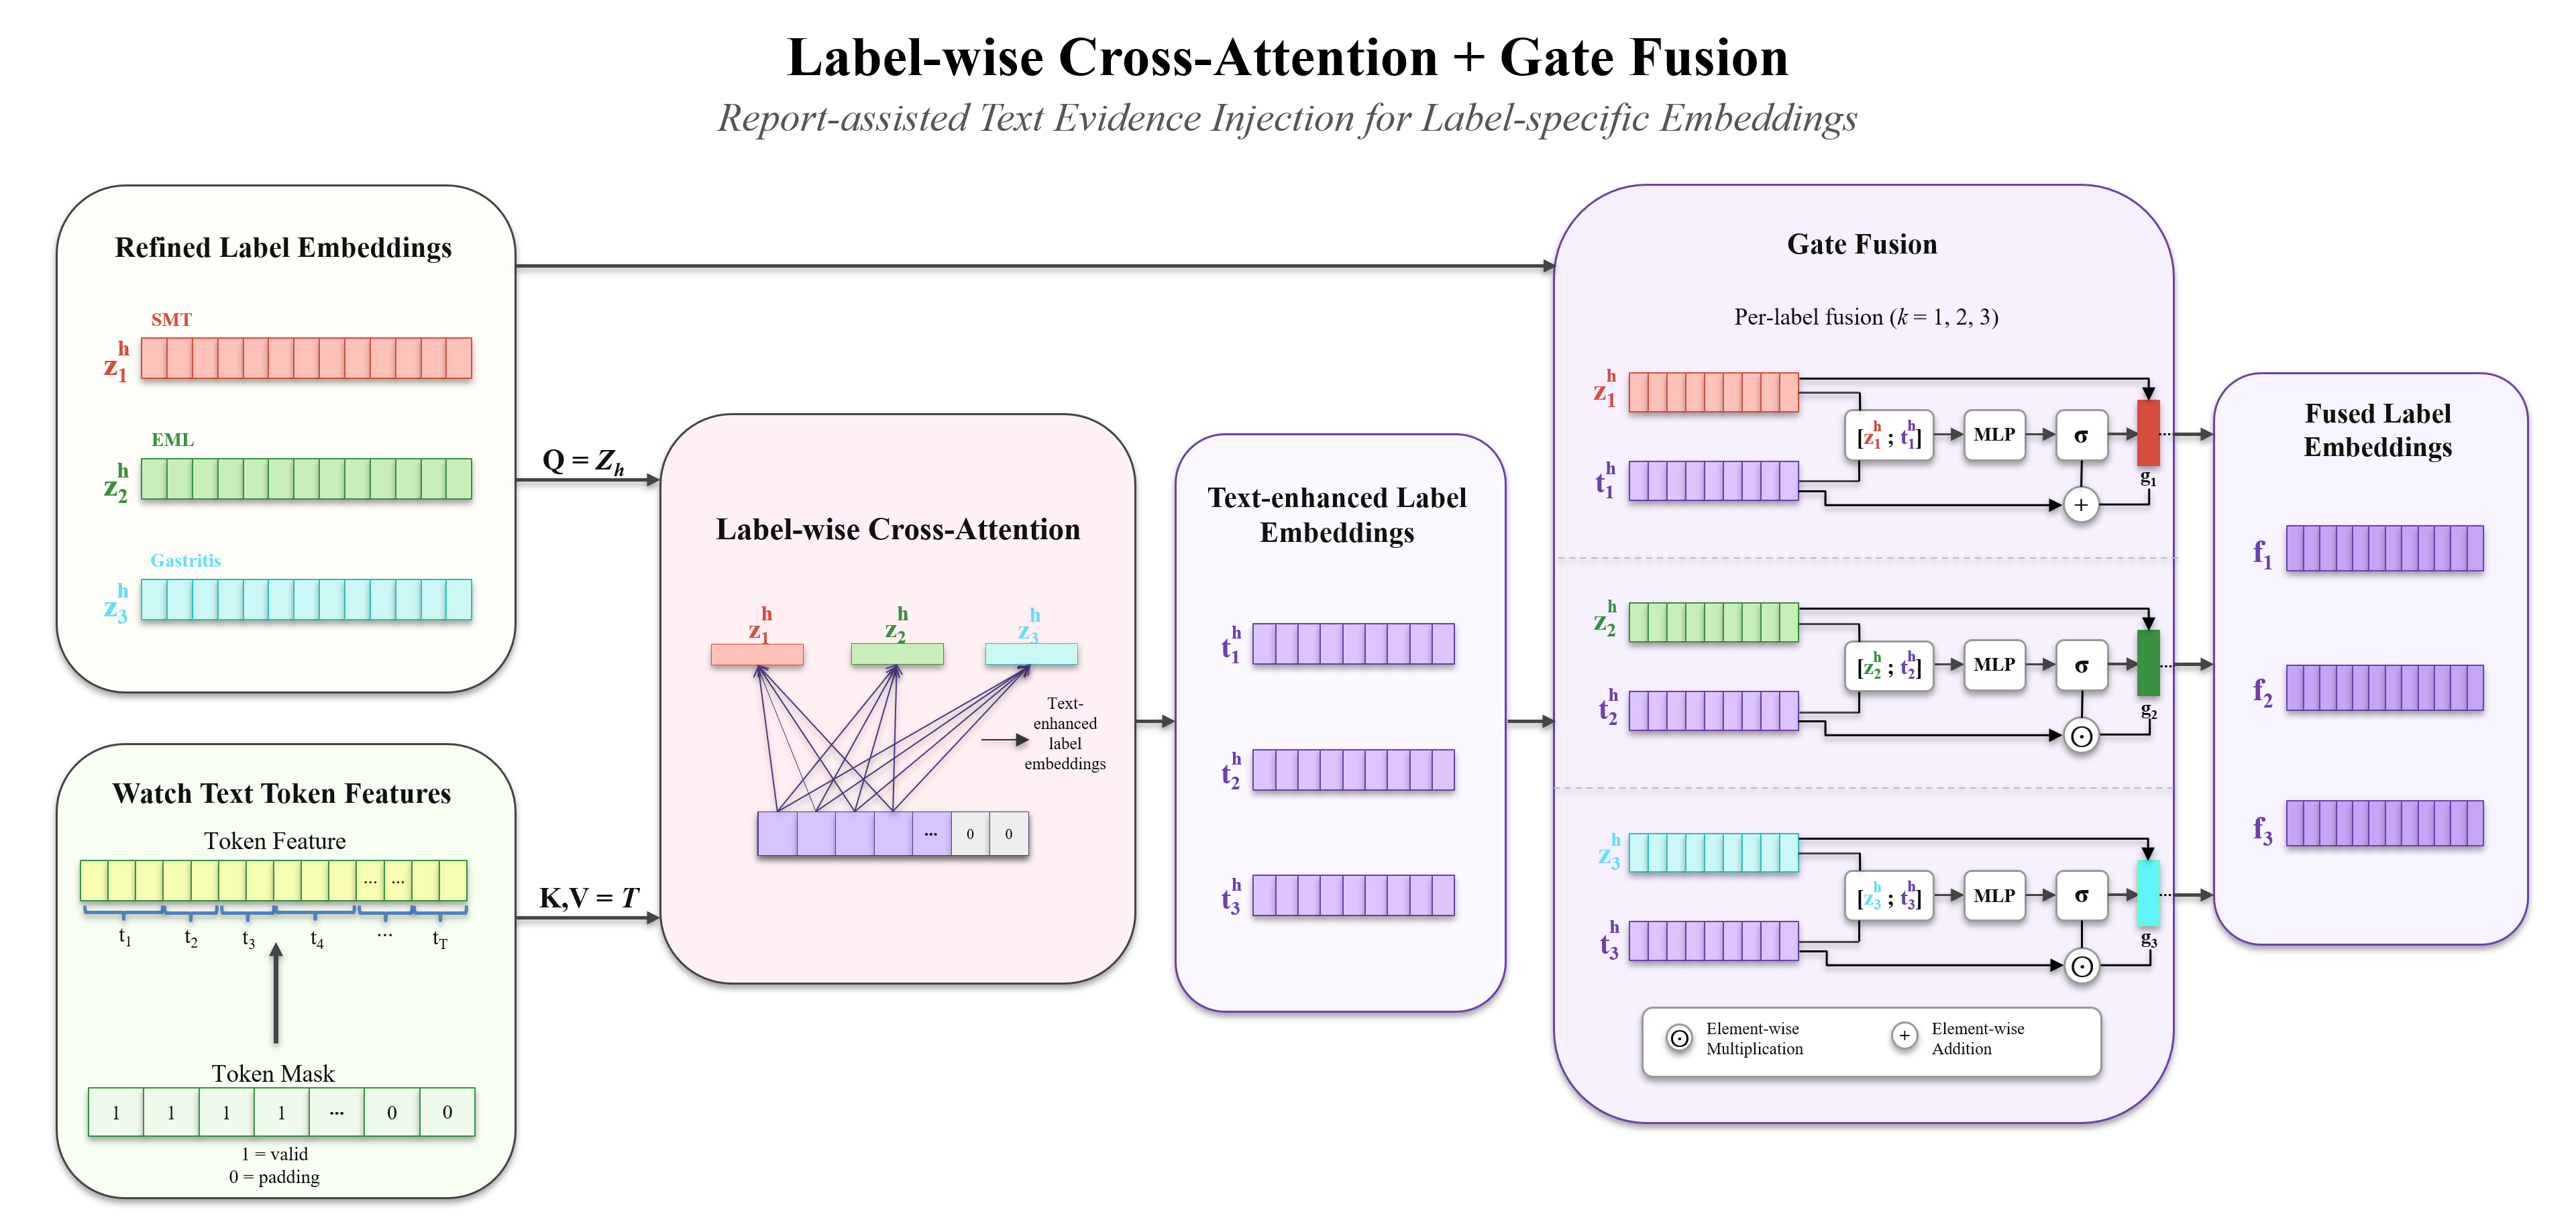
\includegraphics[width=\textwidth]{figs/cross_attention_gated_fusion.png}
\caption{Label-query cross-attention and gated multimodal fusion. Each hypergraph-refined visual label representation retrieves relevant masked-report tokens, and a label-wise gate controls their residual contribution to the final representation.\label{fig:cross_attention_gate}}
\end{figure*}

\subsubsection{Multimodal prediction and training objective}

The classifier $C(\cdot)$ was applied to the fused multimodal representation, producing
\begin{equation}
s_i^{mm}=C(Z_i^{fuse}).
\end{equation}
The multimodal logits $s_i^{mm}$ were optimized with asymmetric loss:\cite{R12}
\begin{equation}
\mathcal{L}=\mathcal{L}_{ASL}(s_i^{mm},y_i).
\end{equation}

\textbf{中文翻译：} 分类器$C(\cdot)$作用于融合后的多模态表征，得到
\begin{equation}
s_i^{mm}=C(Z_i^{fuse}).
\end{equation}
使用asymmetric loss优化多模态logits $s_i^{mm}$：
\begin{equation}
\mathcal{L}=\mathcal{L}_{ASL}(s_i^{mm},y_i).
\end{equation}

\section{Experiments}

\subsection{Experimental Settings}

All experiments were conducted on the patient-independent training, validation, and test sets described above. Images were resized to 224$\times$224 pixels, and ConvNeXt-Tiny was used as the image encoder. The intra-examination context encoder contained two Transformer layers with four attention heads. By default, up to 64 images were uniformly sampled from each examination during training and evaluation.

The model was trained for at most 30 epochs using AdamW with an initial learning rate of $2\times10^{-5}$ and a weight decay of 0.02. The examination-level batch size was 1, and dropout was set to 0.2. The first stage of the image encoder was frozen during training. The asymmetric multi-label loss was used as the classification objective.

For the text-only comparison, five encoders were evaluated using only the category-masked endoscopic finding field: a hashed mean encoder, a vocabulary attention encoder, TextCNN, BiGRU, and a Transformer encoder. These controls used the same patient-independent data split and predicted the same three examination-level labels, allowing direct comparison with the image-only and multimodal settings.

\textbf{中文翻译：} 所有实验均使用前文所述按患者相互独立划分的训练集、验证集和测试集。输入图像被缩放至224$\times$224像素，并采用ConvNeXt-Tiny作为图像编码器。检查内上下文编码器包含2层Transformer和4个注意力头。默认情况下，训练和评估时均从每次检查中均匀采样最多64张图像。

模型使用AdamW训练最多30个epoch，初始学习率为$2\times10^{-5}$，权重衰减为0.02。检查级batch size设为1，dropout设为0.2，并在训练过程中冻结图像编码器的第一阶段。分类目标采用非对称多标签损失。

纯文本对照实验仅使用类别名称掩码后的内镜所见字段，并比较了5种编码器：哈希均值编码器、词表注意力编码器、TextCNN、BiGRU和Transformer编码器。这些对照使用相同的患者独立数据划分，并预测相同的3个检查级标签，从而可与纯图像和多模态设置进行直接比较。

\subsection{Evaluation Protocol}

Predicted probabilities were converted into binary decisions using a fixed threshold of 0.5 for all three labels. Macro F1 was selected as the primary metric because it gives equal importance to each target label, whereas micro F1 summarizes decisions over all examination--label pairs. Macro ROC-AUC and macro PR-AUC were used to evaluate ranking performance. Subset accuracy measured the proportion of examinations for which all three labels were predicted correctly, and hamming loss measured the proportion of incorrect individual label decisions. Cohen's kappa was additionally reported to quantify agreement beyond chance. For each disease, accuracy, recall, precision, specificity, F1, ROC-AUC, and PR-AUC were calculated. All results are point estimates on the fixed internal test set of 567 examinations.

\textbf{中文翻译：} 对三个标签均使用固定阈值0.5将预测概率转换为二值结果。宏平均F1被设为主要指标，因为该指标对每个目标标签赋予相同权重；微平均F1则汇总所有“检查--标签”预测。宏平均ROC-AUC和宏平均PR-AUC用于评价排序性能。子集准确率表示三个标签均预测正确的检查所占比例，汉明损失表示逐标签预测错误的比例。此外，本文报告Cohen's kappa以衡量校正随机一致性后的预测一致程度。对于每种疾病，分别计算准确率、召回率、精确率、特异度、F1、ROC-AUC和PR-AUC。所有结果均为固定内部测试集567次检查上的点估计。

\subsection{Comparison with Image-only and Text-only Models}

To distinguish the contributions of the two input modalities, Table~\ref{T2} compares image-only MIL models, text-only classifiers using the category-masked endoscopic finding field, and the proposed multimodal model. The strongest image-only macro F1 was 0.8606, achieved by Top-$k$ MIL and TransMIL, while TextCNN was the strongest text-only classifier with a macro F1 of 0.8511. MEF-CAH-MIL achieved a macro F1 of 0.8979, exceeding the best image-only and text-only results by 0.0373 and 0.0468, respectively. The consistent improvements in micro F1, subset accuracy, hamming loss, and kappa support the complementary value of combining the complete image bag with masked report findings.

\textbf{中文翻译：} 为区分两种输入模态的贡献，表~\ref{T2}比较了仅使用图像bag的MIL模型、仅使用类别名称掩码后内镜所见文本的分类器，以及本文提出的多模态模型。图像端模型中，Top-$k$ MIL和TransMIL取得最高宏平均F1 0.8606；文本端模型中，TextCNN取得最高宏平均F1 0.8511。MEF-CAH-MIL的宏平均F1为0.8979，分别比最佳图像端和文本端结果高0.0373和0.0468。微平均F1、子集准确率、汉明损失和kappa的同步改善，支持完整图像bag与掩码报告所见之间具有互补价值。

\begin{table*}[t]
\scriptsize\sf\centering
\caption{Comparison of image-only, text-only, and multimodal models on the internal test set. img. and txt. indicate whether image and masked-report text inputs were used, respectively.\label{T2}}
\resizebox{\textwidth}{!}{%
\begin{tabular}{lcc*{7}{c}}
\hline
Model & img. & txt. & \shortstack{Macro\\F1} & \shortstack{Micro\\F1} & \shortstack{Macro\\ROC-AUC} & \shortstack{Macro\\PR-AUC} & \shortstack{Subset\\accuracy} & \shortstack{Hamming\\loss} & Kappa \\
\hline
Attention MIL & $\checkmark$ & $\times$ & 0.8504 & 0.8469 & 0.9179 & 0.9164 & 0.6672 & 0.1556 & 0.6894 \\
Mean pooling & $\checkmark$ & $\times$ & 0.8584 & 0.8555 & 0.9190 & 0.9102 & 0.6742 & 0.1487 & 0.7035 \\
Transformer-context MIL & $\checkmark$ & $\times$ & 0.8589 & 0.8550 & 0.9253 & 0.9181 & 0.6812 & 0.1475 & 0.7057 \\
Top-$k$ MIL & $\checkmark$ & $\times$ & 0.8606 & 0.8559 & 0.9220 & 0.9106 & 0.6620 & 0.1487 & 0.7037 \\
Max pooling & $\checkmark$ & $\times$ & 0.7533 & 0.7398 & 0.8439 & 0.8416 & 0.1533 & 0.3287 & 0.3544 \\
TransMIL & $\checkmark$ & $\times$ & 0.8606 & 0.8583 & 0.9247 & 0.9179 & 0.7143 & 0.1429 & 0.7147 \\
DSMIL & $\checkmark$ & $\times$ & 0.8601 & 0.8570 & 0.9241 & 0.9181 & 0.6951 & 0.1452 & 0.7102 \\
DTFD-MIL & $\checkmark$ & $\times$ & 0.8452 & 0.8405 & 0.9177 & 0.9098 & 0.5714 & 0.1719 & 0.6583 \\
CLAM-MB & $\checkmark$ & $\times$ & 0.8360 & 0.8321 & 0.9071 & 0.9000 & 0.5958 & 0.1760 & 0.6496 \\
CLAM-SB & $\checkmark$ & $\times$ & 0.8284 & 0.8236 & 0.9070 & 0.8907 & 0.5453 & 0.1911 & 0.6203 \\
\hline
Hashed mean encoder & $\times$ & $\checkmark$ & 0.8426 & 0.8441 & 0.9184 & 0.9067 & 0.7019 & 0.1517 & 0.6962 \\
Vocabulary attention encoder & $\times$ & $\checkmark$ & 0.8493 & 0.8508 & 0.9231 & 0.9124 & 0.7152 & 0.1455 & 0.7088 \\
TextCNN encoder & $\times$ & $\checkmark$ & 0.8511 & 0.8524 & 0.9316 & 0.9208 & 0.7213 & 0.1423 & 0.7146 \\
BiGRU encoder & $\times$ & $\checkmark$ & 0.8478 & 0.8490 & 0.9257 & 0.9149 & 0.7125 & 0.1464 & 0.7069 \\
Transformer encoder & $\times$ & $\checkmark$ & 0.8502 & 0.8515 & 0.9294 & 0.9186 & 0.7187 & 0.1437 & 0.7120 \\
\hline
MEF-CAH-MIL & $\checkmark$ & $\checkmark$ & \textbf{0.8979} & \textbf{0.8949} & \textbf{0.9532} & \textbf{0.9362} & \textbf{0.7813} & \textbf{0.1029} & \textbf{0.7945} \\
\hline
\end{tabular}
}
\end{table*}

\subsection{Test-set Confusion Analysis}

Figure~\ref{fig:test_confusion} shows the one-vs-rest confusion matrix for each target at the fixed threshold of 0.5. The final model correctly identified 245 of 265 esophageal submucosal tumor cases, 279 of 310 esophageal mucosal lesion cases, and 221 of 223 gastritis cases. Gastritis had only two false negatives, whereas the two esophageal targets had more false positives (49 and 46, respectively), indicating high sensitivity with comparatively lower specificity for these labels.

\textbf{中文翻译：} 图~\ref{fig:test_confusion}展示了固定阈值0.5下三个目标标签各自的一对其余混淆矩阵。最终模型正确识别了265例食管黏膜下肿瘤中的245例、310例食管粘膜病变中的279例，以及223例胃炎中的221例。胃炎仅出现2例假阴性，而两个食管标签的假阳性相对较多（分别为49例和46例），表明模型对这些标签具有较高敏感度，但特异度相对较低。

\begin{figure*}[t]
\centering
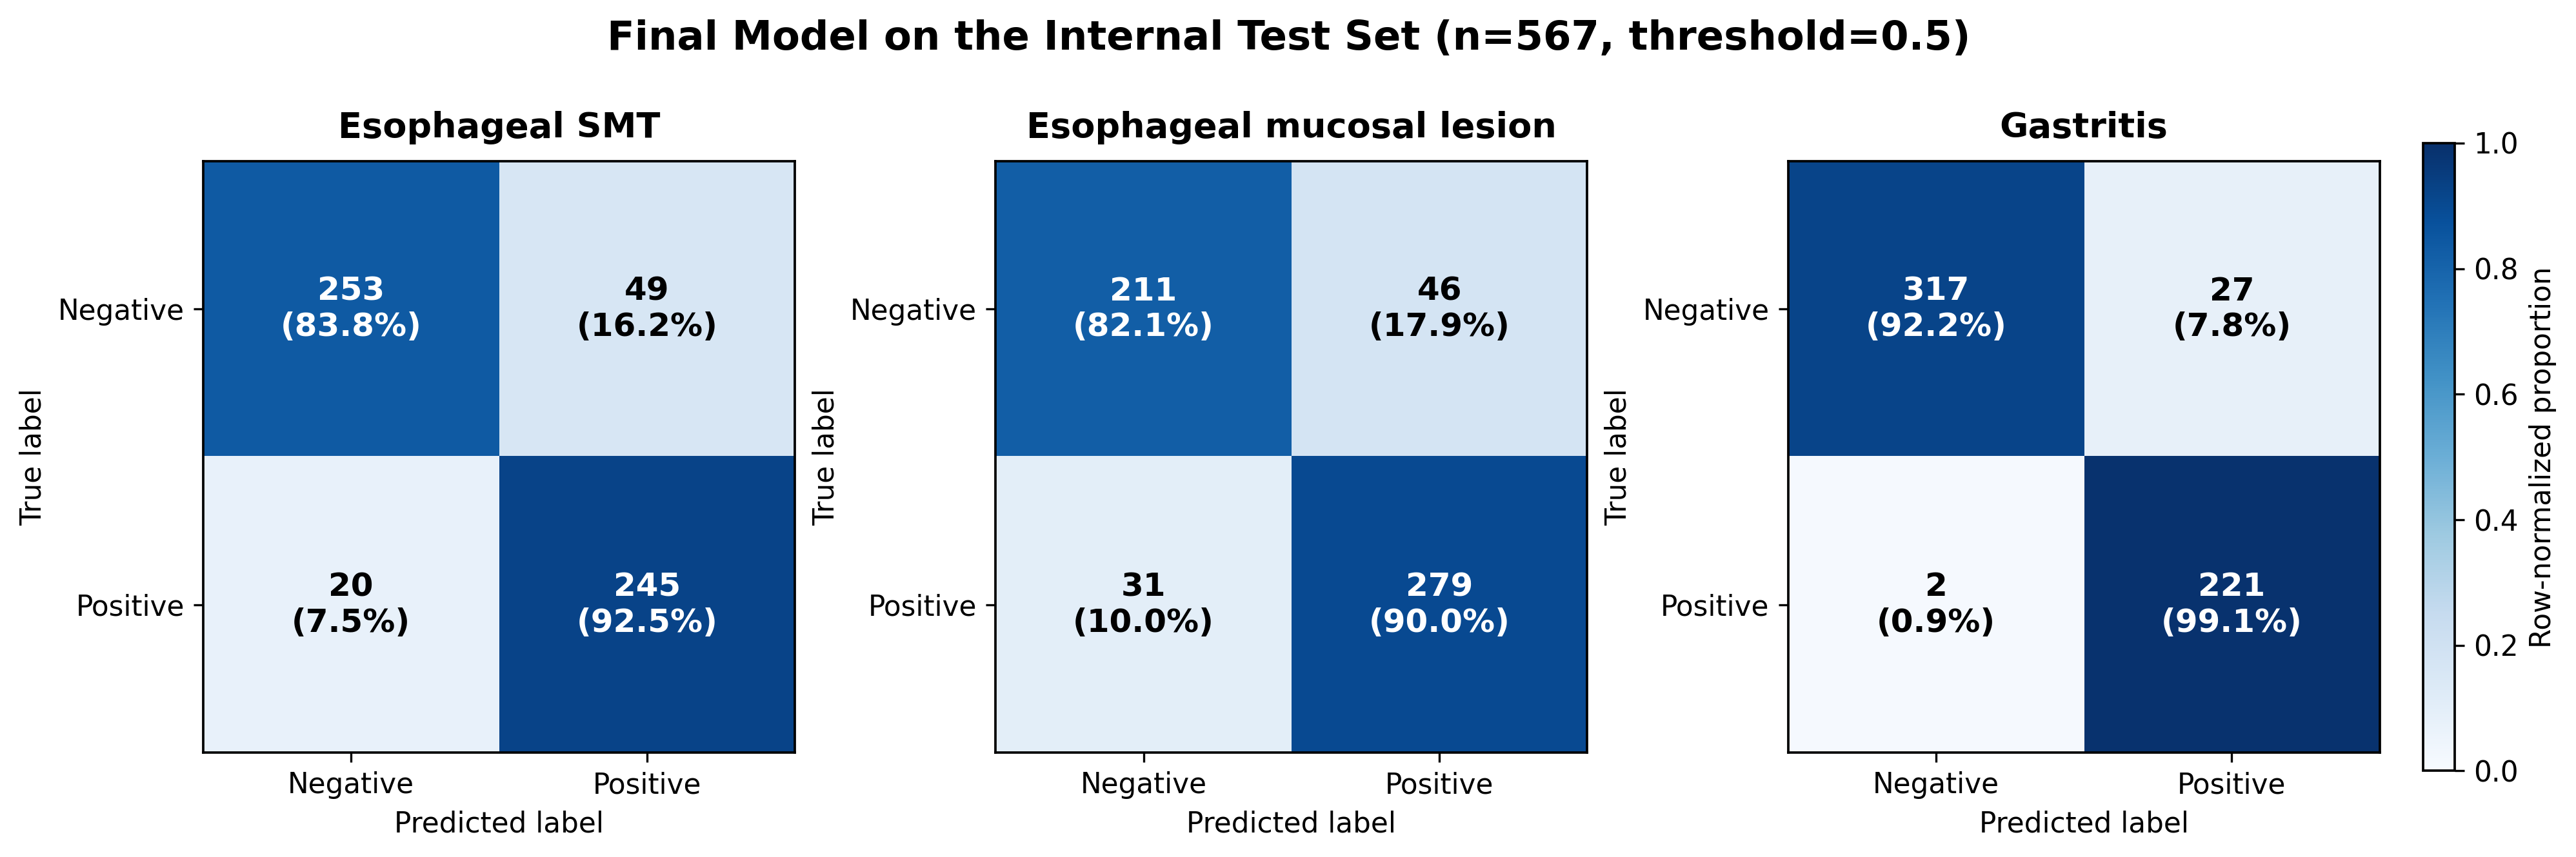
\includegraphics[width=\textwidth]{figs/test_confusion_matrices.png}
\caption{One-vs-rest confusion matrices of the final model on the internal test set ($n=567$) at a threshold of 0.5. Rows denote true classes and columns denote predicted classes; each cell reports the count and its percentage within the corresponding true-class row.\label{fig:test_confusion}}
\end{figure*}

\subsection{Effect of Image Number and Context Modeling}

To examine how the number of sampled images affected examination-level classification, we evaluated models using 16, 32, 48, 64, 80, or 96 images per examination. All settings other than the image budget and the position/context module were kept unchanged. Table~\ref{T3} separates the results into a context-free panel and a position-and-context-enabled panel and reports all seven examination-level metrics. Position and context modeling improved macro F1 at every image budget, with gains ranging from 0.0050 to 0.0163. At 64 images, it increased macro F1 from 0.8816 to 0.8979, micro F1 from 0.8795 to 0.8949, and kappa from 0.7619 to 0.7945, while reducing hamming loss from 0.1193 to 0.1029.

The context-free configuration reached its best macro F1 of 0.8836 with 96 images, whereas the context-enabled configuration reached its best macro F1 of 0.8979 with 64 images. Although the highest context-enabled subset accuracy occurred at 96 images (0.7866), the 64-image setting provided the strongest primary metric and the best values for five of the remaining six metrics. It was therefore retained as the final image budget.

\textbf{中文翻译：} 为分析采样图像数量对检查级分类的影响，本文分别使用每次检查16、32、48、64、80和96张图像进行实验。除图像数量以及位置编码与上下文编码器模块外，其余设置保持一致。表~\ref{T3}将结果分为不使用上下文建模和使用位置编码与上下文编码器两个分区，并报告全部7项检查级指标。位置与上下文建模在所有图像数量下均提高了宏平均F1，增幅为0.0050--0.0163。在64张图像下，该模块将宏平均F1从0.8816提高至0.8979，将微平均F1从0.8795提高至0.8949，将kappa从0.7619提高至0.7945，同时将汉明损失从0.1193降低至0.1029。

不使用上下文建模的配置在96张图像时取得其最高宏平均F1 0.8836，而使用位置编码与上下文编码器的配置在64张图像时取得最高宏平均F1 0.8979。尽管后者的最高子集准确率出现在96张图像时（0.7866），但64张图像在主要指标上最优，并在其余6项指标中的5项取得最佳结果。因此，本文最终采用64张图像作为默认输入数量。

\begin{table*}[t]
\small\sf\centering
\caption{Effect of the image sampling budget with and without position encoding and the intra-examination context encoder. The two panels report all evaluation metrics under otherwise identical settings.\label{T3}}
\resizebox{\textwidth}{!}{%
\begin{tabular}{c*{7}{c}}
\hline
\multicolumn{8}{l}{\textbf{Panel A: Without position encoding and context encoder}} \\
\hline
Images & Macro F1 & Micro F1 & Macro ROC-AUC & Macro PR-AUC & Subset accuracy & Hamming loss & Kappa \\
16 & 0.8673 & 0.8638 & 0.9238 & 0.9021 & 0.7319 & 0.1340 & 0.7324 \\
32 & 0.8743 & 0.8710 & 0.9345 & 0.9207 & 0.7337 & 0.1252 & 0.7496 \\
48 & 0.8720 & 0.8693 & 0.9348 & 0.9159 & 0.7531 & 0.1264 & 0.7471 \\
64 & 0.8816 & 0.8795 & \textbf{0.9409} & 0.9194 & 0.7513 & 0.1193 & 0.7619 \\
80 & 0.8814 & 0.8783 & 0.9370 & 0.9182 & 0.7619 & 0.1182 & 0.7637 \\
96 & \textbf{0.8836} & \textbf{0.8806} & 0.9370 & \textbf{0.9212} & \textbf{0.7672} & \textbf{0.1164} & \textbf{0.7674} \\
\hline
\multicolumn{8}{l}{\textbf{Panel B: With position encoding and context encoder}} \\
\hline
Images & Macro F1 & Micro F1 & Macro ROC-AUC & Macro PR-AUC & Subset accuracy & Hamming loss & Kappa \\
16 & 0.8819 & 0.8789 & 0.9382 & 0.9122 & 0.7178 & 0.1217 & 0.7577 \\
32 & 0.8840 & 0.8797 & 0.9393 & 0.9184 & 0.7266 & 0.1199 & 0.7610 \\
48 & 0.8872 & 0.8849 & 0.9402 & 0.9231 & 0.7672 & 0.1123 & 0.7756 \\
64 & \textbf{0.8979} & \textbf{0.8949} & \textbf{0.9532} & \textbf{0.9362} & 0.7813 & \textbf{0.1029} & \textbf{0.7945} \\
80 & 0.8864 & 0.8837 & 0.9420 & 0.9264 & 0.7531 & 0.1152 & 0.7702 \\
96 & 0.8930 & 0.8906 & 0.9422 & 0.9242 & \textbf{0.7866} & 0.1058 & 0.7883 \\
\hline
\end{tabular}
}
\end{table*}

\subsection{Ablation Study}

\subsubsection{Full-factorial module ablation}

We evaluated all $2^4=16$ combinations of four modules using up to 64 images per examination and random seed 2026. When M2 was disabled, it was replaced by an ordinary learnable label graph. When both M3 and M4 were disabled, the model used the image pathway; M3 alone used cross-attention followed by direct addition, whereas M4 alone used a pooled report representation with a gate. The module definitions are provided in the caption of Table~\ref{T_factorial}.

As shown in Table~\ref{T_factorial}, the no-module baseline achieved a macro F1 of 0.8690. M2, M3, and M4 individually improved macro F1 by 0.63, 1.59, and 1.87 percentage points, respectively, whereas M1 alone produced a negligible change. M2+M4 was the strongest two-module configuration (0.8878). With all four modules enabled, the final model achieved a macro F1 of 0.8979, micro F1 of 0.8949, macro ROC-AUC of 0.9532, subset accuracy of 0.7813, hamming loss of 0.1029, and kappa of 0.7945, giving the best result for six of the seven metrics. M4 alone retained the highest macro PR-AUC of 0.9412. Disabling any one module from the final model reduced macro F1 by 1.03--1.97 percentage points, supporting the complementary contribution of the four components.

\textbf{中文翻译：} 本文使用每次检查最多64张图像和随机种子2026，评估四个模块的全部$2^4=16$种组合。关闭M2时使用普通可学习标签图替代；M3和M4同时关闭时采用图像路径；仅启用M3时使用cross-attention后直接相加，仅启用M4时使用池化报告表征和门控融合。M1--M4的具体含义见表~\ref{T_factorial}表注。

如表~\ref{T_factorial}所示，不使用四个模块的基线宏平均F1为0.8690。单独加入M2、M3和M4后，宏平均F1分别提高0.63、1.59和1.87个百分点，而单独加入M1时变化很小。M2+M4是表现最好的双模块配置（0.8878）。四个模块全部启用时，最终模型的宏平均F1为0.8979、微平均F1为0.8949、宏平均ROC-AUC为0.9532、子集准确率为0.7813、汉明损失为0.1029、kappa为0.7945，在7项指标中的6项取得最优结果；单独使用M4时宏平均PR-AUC最高（0.9412）。从最终模型中关闭任一模块都会使宏平均F1下降1.03--1.97个百分点，说明四个模块具有互补贡献。

\begin{table*}[t]
\footnotesize\sf\centering
\caption{Full-factorial ablation of the four proposed modules on the internal test set. M1: position encoding and Transformer context encoder; M2: label hypergraph learning; M3: label-query cross-attention; M4: gated fusion. All entries use the checkpoint selected by validation macro F1.\label{T_factorial}}
\resizebox{\textwidth}{!}{%
\begin{tabular}{*{4}{c}*{7}{c}}
\hline
M1 & M2 & M3 & M4 & \shortstack{Macro\\F1} & \shortstack{Micro\\F1} & \shortstack{Macro\\ROC-AUC} & \shortstack{Macro\\PR-AUC} & \shortstack{Subset\\accuracy} & \shortstack{Hamming\\loss} & Kappa \\
\hline
-- & -- & -- & -- & 0.8690 & 0.8666 & 0.9350 & 0.9193 & 0.7213 & 0.1323 & 0.7362 \\
$\checkmark$ & -- & -- & -- & 0.8687 & 0.8659 & 0.9269 & 0.9149 & 0.7284 & 0.1311 & 0.7381 \\
-- & $\checkmark$ & -- & -- & 0.8753 & 0.8721 & 0.9357 & 0.9150 & 0.7337 & 0.1264 & 0.7478 \\
-- & -- & $\checkmark$ & -- & 0.8848 & 0.8819 & 0.9391 & 0.9283 & 0.7743 & 0.1146 & 0.7708 \\
-- & -- & -- & $\checkmark$ & 0.8877 & 0.8854 & 0.9507 & \textbf{0.9412} & 0.7707 & 0.1117 & 0.7768 \\
$\checkmark$ & $\checkmark$ & -- & -- & 0.8718 & 0.8706 & 0.9356 & 0.9219 & 0.7443 & 0.1258 & 0.7485 \\
$\checkmark$ & -- & $\checkmark$ & -- & 0.8778 & 0.8742 & 0.9323 & 0.9144 & 0.7460 & 0.1223 & 0.7555 \\
$\checkmark$ & -- & -- & $\checkmark$ & 0.8791 & 0.8749 & 0.9431 & 0.9346 & 0.7637 & 0.1205 & 0.7588 \\
-- & $\checkmark$ & $\checkmark$ & -- & 0.8842 & 0.8812 & 0.9401 & 0.9259 & 0.7707 & 0.1152 & 0.7696 \\
-- & $\checkmark$ & -- & $\checkmark$ & 0.8878 & 0.8848 & 0.9464 & 0.9343 & 0.7478 & 0.1146 & 0.7715 \\
-- & -- & $\checkmark$ & $\checkmark$ & 0.8809 & 0.8785 & 0.9355 & 0.9246 & 0.7760 & 0.1176 & 0.7648 \\
$\checkmark$ & $\checkmark$ & $\checkmark$ & -- & 0.8859 & 0.8835 & 0.9376 & 0.9181 & 0.7566 & 0.1135 & 0.7732 \\
$\checkmark$ & $\checkmark$ & -- & $\checkmark$ & 0.8876 & 0.8854 & 0.9484 & 0.9389 & 0.7654 & 0.1123 & 0.7757 \\
$\checkmark$ & -- & $\checkmark$ & $\checkmark$ & 0.8782 & 0.8752 & 0.9345 & 0.9170 & 0.7460 & 0.1211 & 0.7578 \\
-- & $\checkmark$ & $\checkmark$ & $\checkmark$ & 0.8816 & 0.8795 & 0.9409 & 0.9194 & 0.7513 & 0.1193 & 0.7619 \\
$\checkmark$ & $\checkmark$ & $\checkmark$ & $\checkmark$ & \textbf{0.8979} & \textbf{0.8949} & \textbf{0.9532} & 0.9362 & \textbf{0.7813} & \textbf{0.1029} & \textbf{0.7945} \\
\hline
\end{tabular}
}
\end{table*}

\FloatBarrier

\subsubsection{Selected architectural contrasts}

Selected contrasts in Table~\ref{T_factorial} provide further architectural interpretation. Relative to the final four-module model, disabling both cross-attention and gated fusion reduced macro F1 from 0.8979 to 0.8718, showing that the report-guided fusion pathway provided complementary evidence beyond the image pathway. Replacing the label hypergraph with an ordinary label graph reduced macro F1 to 0.8782. Disabling cross-attention while retaining gated fusion produced a macro F1 of 0.8876 and a slightly higher macro PR-AUC, but lower subset accuracy and kappa than the final model. Disabling the fusion gate reduced macro F1 to 0.8859. These observations support the joint use of hypergraph reasoning, label-query cross-attention, and gated fusion for thresholded multi-label decisions.

\textbf{中文翻译：} 表~\ref{T_factorial}中的代表性配置可以进一步解释各架构的作用。相对于最终四模块模型，同时关闭cross-attention和门控融合后，宏平均F1由0.8979下降至0.8718，说明报告引导的融合路径能够在图像路径之外提供互补证据。将标签超图替换为普通标签图后，宏平均F1下降至0.8782。关闭cross-attention但保留门控融合时，宏平均F1为0.8876，宏平均PR-AUC略高，但子集准确率和kappa低于最终模型。关闭融合门控后，宏平均F1下降至0.8859。这些结果支持联合使用超图推理、标签查询cross-attention和门控融合，以改善阈值化多标签判定。

\FloatBarrier

\section{Discussion}

This study suggests that examination-level gastroscopy classification can benefit from explicitly modeling both multi-image evidence and routine endoscopic finding text. The clinical value of this formulation is that it treats a gastroscopy examination as it is recorded in practice: a variable-length image set accompanied by narrative findings. Compared with a purely image-only formulation, the report-assisted setting more closely resembles workflows in which endoscopic images and procedural descriptions are reviewed together for quality control, follow-up prioritization, or assisted review. The proposed label-query cross-attention mechanism is suitable for this multi-label setting because different labels can retrieve different textual cues and attend to different image evidence within the same examination.

\textbf{中文翻译：} 本研究提示，检查级胃镜分类可以从显式建模多图像证据和常规内镜所见文本中获益。该定义的临床价值在于，它按照真实实践中的记录方式看待一次胃镜检查：一个长度不固定的图像集合，同时伴随叙述性检查所见。与纯图像设定相比，报告辅助设定更接近内镜图像和检查描述共同用于质量控制、随访优先级排序或辅助复核的工作流程。所提出的标签查询cross-attention机制适合这一多标签场景，因为不同标签可以从同一次检查中检索不同文本线索，并关注不同图像证据。

The model achieved the strongest label-wise performance for gastritis and useful performance for both esophageal labels. This pattern is clinically plausible. Gastritis often produces more distributed visual evidence and may also be described explicitly in the \textit{watch} field, whereas esophageal submucosal tumor and esophageal mucosal lesion are more localized and may appear in fewer frames. The relatively higher false-positive burden for esophageal findings should not be viewed only as a numerical limitation; it also points to a clinically important failure mode. Some protrusions, folds, inflammation-related changes, or nonspecific mucosal irregularities may resemble target esophageal findings in individual frames or in narrative wording. Future work should therefore include lesion-level expert review, key-frame annotation, or region-level verification to separate visually ambiguous esophageal findings from true positive disease patterns.

\textbf{中文翻译：} 模型在胃炎标签上取得最强分标签性能，并在两个食管标签上取得有实用意义的表现。这一模式具有临床合理性。胃炎通常产生更广泛分布的视觉证据，也可能在\textit{watch}字段中被明确描述；而食管黏膜下肿瘤和食管粘膜病变更局灶，可能只出现在少数图像帧中。食管相关发现假阳性相对较多，不应仅被看作数值层面的局限，它也提示了一个具有临床意义的错误模式：部分隆起、皱襞、炎症相关改变或非特异性粘膜不规则，可能在单帧图像或报告措辞上接近目标食管发现。因此，未来工作应引入病灶级专家复核、关键帧标注或区域级验证，以区分视觉表现不明确的食管发现与真正阳性疾病模式。

A central issue in this study is the interpretation boundary of report-assisted learning. The model does not use \textit{watchResult}, which is the label-derivation field, but it does use \textit{watch}, which may contain target-related clinical language. Therefore, the model should not be claimed as evidence that images alone are sufficient for the reported performance. Instead, it should be understood as a practical multimodal system that combines images and procedural findings for examination-level decision support. This distinction is important for fair comparison with image-only systems, for regulatory interpretation, and for the design of prospective clinical studies.

\textbf{中文翻译：} 本研究的核心问题之一是报告辅助学习的解释边界。模型未使用作为标签派生来源的\textit{watchResult}字段，但使用了可能包含目标相关临床语言的\textit{watch}字段。因此，不能将模型性能解释为“仅依靠图像即可达到该结果”的证据。更合适的解释是：该模型是一种结合图像和检查所见的实用多模态系统，用于检查级决策支持。这一区分对于与纯图像系统进行公平比较、监管解释以及未来前瞻性临床研究设计都很重要。

\subsection{Limitations and Future Work}

This study has several limitations. First, the data came from a single center, and the model was evaluated only by internal validation. Differences in endoscopy devices, image acquisition habits, report templates, terminology, and patient population may affect generalization. External multi-center validation is required before the model can be considered robust across institutions.

\textbf{中文翻译：} 本研究存在若干局限性。首先，数据来自单中心，模型仅通过内部验证进行评估。不同机构在内镜设备、图像采集习惯、报告模板、术语使用和患者人群方面的差异可能影响模型泛化能力。因此，在认为模型具备跨机构鲁棒性之前，仍需进行外部多中心验证。

Second, the reference labels were derived from routine diagnostic reports rather than independent expert consensus, histopathological confirmation for all cases, or prospective adjudication. This weak-supervision strategy enables scalable learning from real-world archives but may introduce label noise due to reporting variability, incomplete descriptions, or rule-based matching errors.

\textbf{中文翻译：} 第二，参考标签来源于常规诊断报告，而不是所有病例的独立专家共识、组织病理学确认或前瞻性裁定。这种弱监督策略使模型能够从真实世界归档数据中进行可扩展学习，但也可能由于报告差异、不完整描述或规则匹配错误引入标签噪声。

Third, the model uses \textit{watch} during inference. Although this is appropriate for a report-assisted workflow, it may encode part of the diagnostic reasoning already present in the report narrative. The category masking and modality-specific controls reduce this concern but cannot eliminate it. Future work should include stronger leakage audits, external evaluation of text-only controls, image-only student distillation, and prospective workflow studies to quantify how much incremental value the model adds beyond the report text alone.

\textbf{中文翻译：} 第三，模型在推理阶段使用\textit{watch}字段。虽然这适用于报告辅助工作流，但它可能编码报告叙述中已有的部分诊断推理。类别名称掩码和分模态对照能够缓解这一问题，但不能将其完全排除。未来工作应开展更严格的信息泄漏审计、纯文本对照的外部验证、图像单模态学生模型蒸馏以及前瞻性工作流研究，以量化模型相对于单独报告文本所带来的增量价值。

Fourth, although the full-factorial and targeted ablations separate the main architectural contributions, these results are point estimates from a single random seed. More extensive repeated-seed comparisons and confidence intervals for the text-only, multimodal, and ablation estimates are still required to quantify uncertainty and confirm the observed modality differences and module interactions.

\textbf{中文翻译：} 第四，尽管完整全因子消融和关键模块消融区分了主要架构贡献，但这些结果仍是单一随机种子下的点估计。后续仍需开展更多重复随机种子比较，并为纯文本、多模态及消融结果报告置信区间，以量化不确定性并验证观察到的模态差异和模块交互作用。

Finally, interpretability was based on model-derived attention and intermediate outputs rather than expert-validated lesion localization. Attention weights can suggest which images or tokens contributed to predictions, but they do not prove causal decision mechanisms or accurate lesion localization. Future studies should include expert key-frame labels, lesion bounding regions, and systematic failure-case review.

\textbf{中文翻译：} 最后，可解释性主要基于模型生成的注意力和中间输出，而不是专家验证的病灶定位。注意力权重可以提示哪些图像或token对预测有贡献，但不能证明因果决策机制或准确病灶定位。未来研究应纳入专家关键帧标签、病灶区域标注和系统性失败病例复核。

\section{Conclusions}

In this retrospective single-center study, we developed and internally validated \textit{MEF-CAH-MIL}, a multimodal endoscopic finding-guided cross-attentive hypergraph multiple instance learning framework for examination-level multi-label classification of gastroscopy. The method integrates up to 64 endoscopic images with routine endoscopic finding text, uses label-query cross-attention and gated fusion to produce label-specific multimodal representations, and applies label hypergraph reasoning to model relationships among coexisting findings. On the internal test set, the model achieved strong overall and label-wise performance for esophageal submucosal tumor, esophageal mucosal lesion, and gastritis, and outperformed the evaluated image-only and text-only controls. The main value of the framework is that it organizes routine gastroscopy archives into a clinically realistic multimodal, examination-level learning problem. Because the model is report-assisted and has been evaluated only internally, the results should be interpreted as promising evidence of feasibility rather than readiness for clinical deployment. Larger external cohorts, prospective evaluation, and repeated comparisons with modality-specific systems are needed before clinical use.

\textbf{中文翻译：} 在这项回顾性单中心研究中，我们开发并内部验证了\textit{MEF-CAH-MIL}，一种用于胃镜检查级多标签分类的多模态内镜所见引导cross-attentive hypergraph多实例学习框架。该方法融合每次检查最多64张内镜图像与常规内镜所见文本，利用标签查询cross-attention和门控融合生成标签特异性多模态表征，并通过标签超图推理建模共存发现之间的关系。在内部测试集上，模型在食管黏膜下肿瘤、食管粘膜病变以及胃炎三个标签上取得了较强的总体和分标签性能，并优于所评估的纯图像与纯文本对照。该框架的主要价值在于，它将常规胃镜归档数据组织为更贴近临床真实结构的多模态检查级学习问题。由于模型具有报告辅助属性，且目前仅完成内部验证，因此结果应被解释为可行性的积极证据，而不是已经可以临床部署。临床使用前仍需更大规模外部队列、前瞻性评估，以及与分模态系统进行重复比较。

\section*{Author contributions}

Zijian Lin conceived the study, designed the computational framework, implemented the data processing and model training pipeline, performed the experiments, analyzed the results, and drafted the manuscript. Chengze Cai contributed to model design, experimental planning, and manuscript revision. Chenxi Huang provided academic supervision and methodological guidance. Hua Gao and Jie He provided clinical supervision, data access coordination, and interpretation of clinical relevance. All authors reviewed and approved the manuscript.

\textbf{中文翻译：} 林子建构思本研究，设计计算框架，实现数据处理和模型训练流程，完成实验，分析结果并起草论文。蔡成泽参与模型设计、实验规划和论文修改。黄晨曦提供学术监督和方法学指导。高华和何杰提供临床监督、数据获取协调以及临床意义解释。所有作者均审阅并批准本文。

\section*{ORCID iDs}
Zijian Lin \href{https://orcid.org/0009-0007-7260-4064}{0009-0007-7260-4064}\\
Chengze Cai \href{https://orcid.org/0009-0000-8851-1005}{0009-0000-8851-1005}\\
Chenxi Huang \href{https://orcid.org/0000-0002-6695-753X}{0000-0002-6695-753X}\\
Hua Gao \href{https://orcid.org/0009-0007-9844-998X}{0009-0007-9844-998X}\\
Jie He \href{https://orcid.org/0009-0000-6423-3928}{0009-0000-6423-3928}

\textbf{中文翻译：} 作者 ORCID 如上所示。

\section*{Statements and declarations}
\subsection*{Ethical considerations}

This retrospective study used de-identified clinical archive data provided with permission from Zhongshan Hospital (Xiamen), Fudan University. The analysis did not use directly identifiable personal information.

\textbf{中文翻译：} 本回顾性研究使用复旦大学附属中山医院厦门医院授权提供的去标识化临床归档数据。分析过程中未使用可直接识别个人身份的信息。

\subsection*{Consent for publication}

Not applicable because no directly identifiable personal details are reported in this draft manuscript.

\textbf{中文翻译：} 不适用，因为本稿件未报告可直接识别个人身份的信息。

\begin{dci}
The author(s) declared no potential conflicts of interest with respect to the research, authorship, and/or publication of this article.
\end{dci}

\textbf{中文翻译：} 作者声明不存在与本文研究、作者身份和/或发表相关的潜在利益冲突。

\begin{funding}
This work was supported by the Natural Science Foundation of Fujian Province (No. 2025J011511).
\end{funding}

\textbf{中文翻译：} 本研究受到福建省自然科学基金资助（No. 2025J011511）。

\subsection*{Data availability}

The raw gastroscopy images and clinical report data are not publicly available because they may contain sensitive clinical information and are subject to hospital data governance requirements. De-identified derived data tables and code may be made available from the corresponding author on reasonable request and with permission from the hospital.

\textbf{中文翻译：} 原始胃镜图像和临床报告数据由于可能包含敏感临床信息，并受医院数据治理要求约束，因此不公开提供。经去标识化的衍生数据表和代码可在合理请求且获得医院许可后向通讯作者获取。

\begin{acks}
The authors have no acknowledgements to declare.
\end{acks}

\textbf{中文翻译：} 作者无致谢内容需要声明。

\begin{thebibliography}{99}

\bibitem{R2}
Takiyama H, Ozawa T, Ishihara S, Fujishiro M, Shichijo S, Nomura S, Miura M and Tada T. Automatic anatomical classification of esophagogastroduodenoscopy images using deep convolutional neural networks. \textit{Scientific Reports} 2018; 8: 7497.

\bibitem{R3}
Hirasawa T, Aoyama K, Tanimoto T, Ishihara S, Shichijo S, Ozawa T, et al. Application of artificial intelligence using a convolutional neural network for detecting gastric cancer in endoscopic images. \textit{Gastric Cancer} 2018; 21: 653--660.

\bibitem{R4}
Pogorelov K, Randel KR, Griwodz C, de Lange T, Eskeland S, Johansen D, et al. Kvasir: A multi-class image dataset for computer aided gastrointestinal disease detection. In: \textit{Proceedings of the 8th ACM on Multimedia Systems Conference}. 2017, pp. 164--169.

\bibitem{R5}
Borgli H, Thambawita V, Smedsrud PH, Hicks S, Jha D, Eskeland S, et al. HyperKvasir, a comprehensive multi-class image and video dataset for gastrointestinal endoscopy. \textit{Scientific Data} 2020; 7: 283.

\bibitem{R6}
Ilse M, Tomczak JM and Welling M. Attention-based deep multiple instance learning. In: \textit{Proceedings of the 35th International Conference on Machine Learning}. 2018, pp. 2127--2136.

\bibitem{R7}
Lu MY, Williamson DFK, Chen TY, Chen RJ, Barbieri M and Mahmood F. Data-efficient and weakly supervised computational pathology on whole-slide images. \textit{Nature Biomedical Engineering} 2021; 5: 555--570.

\bibitem{R8}
Li B, Li Y and Eliceiri KW. Dual-stream multiple instance learning network for whole slide image classification with self-supervised contrastive learning. In: \textit{Proceedings of the IEEE/CVF Conference on Computer Vision and Pattern Recognition}. 2021, pp. 14318--14328.

\bibitem{R9}
Shao Z, Bian H, Chen Y, Wang Y, Zhang J, Ji X, et al. TransMIL: Transformer based correlated multiple instance learning for whole slide image classification. In: \textit{Advances in Neural Information Processing Systems}. 2021.

\bibitem{R10}
Zhang H, Meng Y, Zhao Y, Qiao Y, Yang X, Coupland SE and Zheng Y. DTFD-MIL: Double-tier feature distillation multiple instance learning for histopathology whole slide image classification. In: \textit{Proceedings of the IEEE/CVF Conference on Computer Vision and Pattern Recognition}. 2022, pp. 18802--18812.

\bibitem{R11}
Liu Z, Mao H, Wu CY, Feichtenhofer C, Darrell T and Xie S. A ConvNet for the 2020s. In: \textit{Proceedings of the IEEE/CVF Conference on Computer Vision and Pattern Recognition}. 2022, pp. 11976--11986.

\bibitem{R12}
Ridnik T, Ben-Baruch E, Zamir N, Noy A, Friedman I, Protter M and Zelnik-Manor L. Asymmetric loss for multi-label classification. In: \textit{Proceedings of the IEEE/CVF International Conference on Computer Vision}. 2021, pp. 82--91.

\bibitem{R13}
Vaswani A, Shazeer N, Parmar N, Uszkoreit J, Jones L, Gomez AN, et al. Attention is all you need. In: \textit{Advances in Neural Information Processing Systems}. 2017.

\bibitem{R14}
Chen ZM, Wei XS, Wang P and Guo Y. Multi-label image recognition with graph convolutional networks. In: \textit{Proceedings of the IEEE/CVF Conference on Computer Vision and Pattern Recognition}. 2019, pp. 5177--5186.

\bibitem{R15}
Li J, Selvaraju RR, Gotmare AD, Joty S, Xiong C and Hoi SCH. Align before fuse: Vision and language representation learning with momentum distillation. In: \textit{Advances in Neural Information Processing Systems}. 2021.

\bibitem{R16}
Li J, Li D, Xiong C and Hoi S. BLIP: Bootstrapping language-image pre-training for unified vision-language understanding and generation. In: \textit{Proceedings of the International Conference on Machine Learning}. 2022.

\bibitem{R17}
Huang SC, Shen L, Lungren MP and Yeung S. GLoRIA: A multimodal global-local representation learning framework for label-efficient medical image recognition. In: \textit{Proceedings of the IEEE/CVF International Conference on Computer Vision}. 2021, pp. 3942--3951.

\bibitem{R18}
Feng Y, You H, Zhang Z, Ji R and Gao Y. Hypergraph neural networks. In: \textit{Proceedings of the AAAI Conference on Artificial Intelligence}. 2019; 33: 3558--3565.

\bibitem{R19}
Luo H, Xu G, Li C, He L, Luo L, Wang Z, et al. Real-time artificial intelligence for detection of upper gastrointestinal cancer by endoscopy: a multicentre, case-control, diagnostic study. \textit{The Lancet Oncology} 2019; 20: 1645--1654.

\bibitem{R20}
Wu L, Zhang J, Zhou W, An P, Shen L, Liu J, et al. Randomised controlled trial of WISENSE, a real-time quality improving system for monitoring blind spots during esophagogastroduodenoscopy. \textit{Gut} 2019; 68: 2161--2169.

\bibitem{R21}
Jha D, Ali S, Hicks S, Thambawita V, Borgli H, Smedsrud PH, et al. A comprehensive analysis of classification methods in gastrointestinal endoscopy imaging. \textit{Medical Image Analysis} 2021; 70: 102007.

\bibitem{R22}
Campanella G, Hanna MG, Geneslaw L, Miraflor A, Silva VWK, Busam KJ, et al. Clinical-grade computational pathology using weakly supervised deep learning on whole slide images. \textit{Nature Medicine} 2019; 25: 1301--1309.

\bibitem{R23}
Zhang Y, Jiang H, Miura Y, Manning CD and Langlotz CP. Contrastive learning of medical visual representations from paired images and text. In: \textit{Proceedings of Machine Learning Research}. 2022; 182: 1--24.

\bibitem{R24}
Zhou HY, Chen X, Zhang Y, Luo R, Wang L and Yu Y. Generalized radiograph representation learning via cross-supervision between images and free-text radiology reports. \textit{Nature Machine Intelligence} 2022; 4: 32--40.

\bibitem{R25}
Buendgens L, Cifci D, Ghaffari Laleh N, van Treeck M, Koenen MT, Zimmermann HW, et al. Weakly supervised end-to-end artificial intelligence in gastrointestinal endoscopy. \textit{Scientific Reports} 2022; 12: 4829.

\bibitem{R26}
Bravo D, Frias J, Vera F, Trejos J, Martinez C, Gomez M, et al. GastroHUN an endoscopy dataset of complete systematic screening protocol for the stomach. \textit{Scientific Data} 2025; 12: 102.

\end{thebibliography}

\end{document}
